% todo: verificar 1,3BD ou 1,3-BD
% todo: verificar seção por seção se as imagens são melhores h, ht, htb
% todo: alterar a legenda das figuras muito compridas
\documentclass[
	% -- opções da classe memoir --
	12pt,				% tamanho da fonte
	openright,			% capítulos começam em pág ímpar (insere página vazia caso preciso)
	twoside,			% para impressão em recto e verso. Oposto a oneside
	a4paper,			% tamanho do papel. 
	% -- opções da classe abntex2 --
	%chapter=TITLE,		% títulos de capítulos convertidos em letras maiúsculas
	%section=TITLE,		% títulos de seções convertidos em letras maiúsculas
	%subsection=TITLE,	% títulos de subseções convertidos em letras maiúsculas
	%subsubsection=TITLE,% títulos de subsubseções convertidos em letras maiúsculas
	% -- opções do pacote babel --
	english,			% idioma adicional para hifenização
	brazil%,				% o último idioma é o principal do documento
%	sumario=tradicional
	]{abntex2}

%%%%%%%%%%%%%%%%%%%%%%%%%%%%%%%%%%%%%%
% Fontes
%\usepackage{lmodern}			% Usa a fonte Latin Modern			
%\usepackage[T1]{fontenc}		% Selecao de codigos de fonte.
%\usepackage[utf8]{inputenc}		% Codificacao do documento (conversão automática dos acentos)
%%%%%%%%%%%%%%%%%%%%%%%%%%
\usepackage{fontspec}
\usepackage{polyglossia}
\setmainlanguage{brazil}
\PolyglossiaSetup{brazil}{indentfirst=true}
\setotherlanguages{english}

\setmainfont[Ligatures=TeX]{Latin Modern Roman}
\setsansfont[Ligatures=TeX]{Latin Modern Sans}
\setmonofont{Latin Modern Mono} 
%%%%%%%%%%%%%%%%%%%%%%%%%
% ABNTEX2
\usepackage{lastpage}			% Usado pela Ficha catalográfica
% \usepackage{indentfirst}		% Indenta o primeiro parágrafo de cada seção.
% \usepackage{color}				% Controle das cores
\usepackage{graphicx}			% Inclusão de gráficos
\DeclareGraphicsExtensions{.pdf, .png}
\usepackage{microtype} 			% para melhorias de justificação
%%%%%%%%%%%%%%%%%%%%%%%%%%
% Meus pacotes
% Matemática
\usepackage{csquotes}
\usepackage{amsmath, amsfonts, amssymb}
\usepackage[makeroom]{cancel}
\usepackage{xfrac}
%\usepackage{nicefrac}
% Cores
\usepackage{xcolor}
\usepackage{enumitem}
% Tabelas
\usepackage{longtable}
\usepackage{booktabs}
\usepackage{multirow}
\usepackage{adjustbox}

\usepackage{lineno}
\renewcommand\linenumberfont{\texttt\tiny}

%\usepackage{float}
%\floatstyle{plaintop} % tabelas com legenda na parte de cima
%\restylefloat{longtable}  % tabelas com legenda na parte de cima

% Figuras
\usepackage[labelsep=period]{caption} % figuras com subfiguras
\usepackage{subcaption}  % figuras com subfiguras
\usepackage{placeins}
\graphicspath{{./figuras}}

% Se eles reclamarem do espaço em branco antes e depois do \part, utilizar titlesec, https://ctan.org/pkg/titlesec, em especial o comando \titlespacing*

% Python
\usepackage{minted}
\setminted[python]{mathescape,
	linenos,
	numbersep=5pt,
	stepnumber=5,
	style=friendly,
	gobble=0,
	baselinestretch=0.5,
	frame=lines,
	framesep=2mm,
	breakautoindent=true,
	breakanywhere=true,
	breaklines=true,
	python3=True,
	texcomments=true}
% https://www.sharelatex.com/learn/Code_Highlighting_with_minted
\renewcommand{\listingscaption}{Código}
\renewcommand{\listoflistingscaption}{Lista de códigos}

\newcommand{\mM}{mmol.L\textsuperscript{-1}}
\newcommand{\Sal}{Sal\textsuperscript{--}}
\newcommand{\q}{\(q\)}
\newcommand{\menosUm}{\textsuperscript{-1}}
\newcommand{\cmc}{CMC}
\newcommand{\cwlm}{\(\mathrm{C}_{\mathrm{WLM}}\)}
\newcommand{\CTAB}{C\textsubscript{16}TAB}
\newcommand{\TTAB}{C\textsubscript{14}TAB}
\newcommand{\DTAB}{C\textsubscript{12}TAB}
\newcommand{\BD}{1,3-BD}  % todo: substituir isso no texto
\newcommand{\CTDTAB}{C\textsubscript{16,14,12}TAB}
\newcommand{\CTTAB}{C\textsubscript{16,14}TAB}
\newcommand{\DHmic}{\(\Delta H^\circ_{\mathrm{mic}}\)}
\newcommand{\DHwlm}{\(\Delta H^\circ_{\mathrm{WLM}}\)}
\newcommand{\figheight}{0.3\textheight}
\newcommand{\agua}{H\textsubscript{2}O}

\renewcommand{\sin}{\hspace{2pt}\mathrm{sen}}
%\renewcommand{\tan}{\hspace{2pt}\mathrm{tg}}

% ---
% Pacotes adicionais, usados apenas no âmbito do Modelo Canônico do abnteX2
% ---
\usepackage{lipsum}				% para geração de dummy text
% ---

% ---
% Pacotes de citações
% ---
\usepackage[brazilian,hyperpageref]{backref}	 % Paginas com as citações na bibl
\usepackage[num]{abntex2cite}	% Citações padrão ABNT
\usepackage{notoccite} % impede de colocar números na LOF e tal

%\usepackage[style=chem-acs, backend=biber,sorting=none,hyperref=true]{biblatex}
%\addbibresource{library.bib}
% --- 
% CONFIGURAÇÕES DE PACOTES
% --- 

%% ---
%% Configurações do pacote backref
%% Usado sem a opção hyperpageref de backref
%\renewcommand{\backrefpagesname}{Citado na(s) página(s):~}
%% Texto padrão antes do número das páginas
%\renewcommand{\backref}{}
%% Define os textos da citação
%\renewcommand*{\backrefalt}[4]{
%	\ifcase #1 %
%		Nenhuma citação no texto.%
%	\or
%		Citado na página #2.%
%	\else
%		Citado #1 vezes nas páginas #2.%
%	\fi}%
%% ---

% ---
% Informações de dados para CAPA e FOLHA DE ROSTO
% ---
\titulo{Estudo estrutural, termodinâmico e cinético sobre a formação e interações de micelas gigantes em sistemas aquosos binários}
\autor{Karl Jan Clinckspoor}
\local{Brasil}
\data{\today}
\orientador{Prof. Dr. Edvaldo Sabadini}
\coorientador{}
\instituicao{%
  Universidade Estadual de Campinas
  \par
  Instituto de Química
  \par
  Programa de Pós-Graduação}
\tipotrabalho{Tese (Doutorado)}
% O preambulo deve conter o tipo do trabalho, o objetivo, 
% o nome da instituição e a área de concentração 
\preambulo{Tese de doutorado realizado no Instituto de Química da Unicamp, na área de Físico-Química, que visa estudar micelas gigantes, sua formação, seu crescimento e as interações intermicelares em sistemas aquosos binários}
% ---


% ---
% Configurações de aparência do PDF final

% alterando o aspecto da cor azul
\definecolor{blue}{RGB}{41,5,195}

% informações do PDF
\makeatletter
\hypersetup{
     	%pagebackref=true,
		pdftitle={\@title}, 
		pdfauthor={\@author},
    	pdfsubject={\imprimirpreambulo},
	    pdfcreator={LaTeX with abnTeX2},
		pdfkeywords={abnt}{latex}{abntex}{abntex2}{trabalho acadêmico}, 
		colorlinks=true,       		% false: boxed links; true: colored links
    	linkcolor=blue,          	% color of internal links
    	citecolor=blue,        		% color of links to bibliography
    	filecolor=magenta,      		% color of file links
		urlcolor=blue,
		bookmarksdepth=4
}
\makeatother
% --- 

% --- 
% Espaçamentos entre linhas e parágrafos 
% --- 

% O tamanho do parágrafo é dado por:
\setlength{\parindent}{1.3cm}

% Controle do espaçamento entre um parágrafo e outro:
\setlength{\parskip}{0.2cm}  % tente também \onelineskip

% ---
% compila o indice
% ---
\makeindex
% ---

% ----
% Início do documento
% ----
%\includeonly{teoria}
\begin{document}

% Retira espaço extra obsoleto entre as frases.
\frenchspacing 

% ----------------------------------------------------------
% ELEMENTOS PRÉ-TEXTUAIS
% ----------------------------------------------------------
% \pretextual

% ---
% Capa
% ---
\imprimircapa
% ---

% ---
% Folha de rosto
% (o * indica que haverá a ficha bibliográfica)
% ---
\imprimirfolhaderosto*
% ---

% ---
% Inserir a ficha bibliografica
% ---

% Isto é um exemplo de Ficha Catalográfica, ou ``Dados internacionais de
% catalogação-na-publicação''. Você pode utilizar este modelo como referência. 
% Porém, provavelmente a biblioteca da sua universidade lhe fornecerá um PDF
% com a ficha catalográfica definitiva após a defesa do trabalho. Quando estiver
% com o documento, salve-o como PDF no diretório do seu projeto e substitua todo
% o conteúdo de implementação deste arquivo pelo comando abaixo:
%
% \begin{fichacatalografica}
%     \includepdf{fig_ficha_catalografica.pdf}
% \end{fichacatalografica}

\begin{fichacatalografica}
	\sffamily
	\vspace*{\fill}					% Posição vertical
	\begin{center}					% Minipage Centralizado
	\fbox{\begin{minipage}[c][8cm]{13.5cm}		% Largura
	\small
	\imprimirautor
	%Sobrenome, Nome do autor
	
	\hspace{0.5cm} \imprimirtitulo  / \imprimirautor. --
	\imprimirlocal, \imprimirdata-
	
	\hspace{0.5cm} \pageref{LastPage} p. : il. (algumas color.) ; 30 cm.\\
	
	\hspace{0.5cm} \imprimirorientadorRotulo~\imprimirorientador\\
	
	\hspace{0.5cm}
	\parbox[t]{\textwidth}{\imprimirtipotrabalho~--~\imprimirinstituicao,
	\imprimirdata.}\\
	
	\hspace{0.5cm}
		1. Surfactantes.
		2. Micelas gigantes.
		2. Reologia.
		I. Edvaldo Sabadini.
		II. Universidade Campinas.
		III. Instituto de Química.
		IV. \imprimirtitulo		
	\end{minipage}}
	\end{center}
\end{fichacatalografica}
% ---

% ---
% Inserir errata
%% ---
%\begin{errata}

%\end{errata}
% ---

% ---
% Inserir folha de aprovação
% ---

% Isto é um exemplo de Folha de aprovação, elemento obrigatório da NBR
% 14724/2011 (seção 4.2.1.3). Você pode utilizar este modelo até a aprovação
% do trabalho. Após isso, substitua todo o conteúdo deste arquivo por uma
% imagem da página assinada pela banca com o comando abaixo:
%
% \includepdf{folhadeaprovacao_final.pdf}
%
\begin{folhadeaprovacao}
%
  \begin{center}
    {\ABNTEXchapterfont\large\imprimirautor}

    \vspace*{\fill}\vspace*{\fill}
    \begin{center}
      \ABNTEXchapterfont\bfseries\Large\imprimirtitulo
    \end{center}
    \vspace*{\fill}
    
    \hspace{.45\textwidth}
    \begin{minipage}{.5\textwidth}
        \imprimirpreambulo
    \end{minipage}%
    \vspace*{\fill}
   \end{center}
        
   %Trabalho aprovado. \imprimirlocal, 24 de novembro de 2012:

   \assinatura{\textbf{\imprimirorientador} \\ Orientador} 
   \assinatura{\textbf{Professor} \\ Convidado 1}
   \assinatura{\textbf{Professor} \\ Convidado 2}
   \assinatura{\textbf{Professor} \\ Convidado 3}
   \assinatura{\textbf{Professor} \\ Convidado 4}
      
   \begin{center}
    \vspace*{0.5cm}
    {\large\imprimirlocal}
    \par
    {\large\imprimirdata}
    \vspace*{1cm}
  \end{center}
  
\end{folhadeaprovacao}
% ---

% ---
% Dedicatória
% ---
\begin{dedicatoria}
   \vspace*{\fill}
   \centering
   \noindent
   \textit{
   	Este trabalho é dedicado ao meu saudoso pai, Guido, que me inspirou a mergulhar na Química, e à minha mãe, Hiris, que me ensinou todo o resto.   
} \vspace*{\fill}
\end{dedicatoria}
% ---

% ---
% Agradecimentos
% ---
\begin{agradecimentos}

Agradeço à minha mãe, a quem amo muito, por ter sempre me apoiado em toda minha vida. Agradeço à Karen, minha maravilhosa namorada, pelo suporte emocional e por compartilhar comigo muitos momentos singelos. Agradeço à Lia, por ter sido uma ótima companhia, desde o início da graduação.

Agradeço ao Prof. Edvaldo, que dirigiu e focou minha atenção, e me apoiou nas diversas decisões que eu tive que tomar durante minha pós graduação. Agradeço ao Prof. Heinz Hoffmann pela paciência, por tantas discussões científicas, e por ter me abrigado em sua casa por uma semana em setembro de 2018. Agradeço ao Prof. Jan Skov Pedersen, por ter aceitado me receber em seu laboratório por um mês em setembro de 2017, mesmo eu sendo um completo amador em SAXS, e depois tendo me ensinado muito sobre a área. Agradeço ao professor René Nome por ter me auxiliado muito nas medidas de cinética por fluorescência.

Agradeço aos colegas e ex-colegas do laboratório B145, pelas discussões e companhia durante esses anos.

Agradeço ao CNPq pelo financiamento.

\end{agradecimentos}
% ---

% ---
% Epígrafe
% --- 
% todo: pensar numa boa epígrafe
\begin{epigrafe}
    \vspace*{\fill}
	\begin{flushright}
		%\textit{''his old life lay behind in the mists, dark adventure lay in front.}
		\textit{``All have their worth and each contributes to the worth of the others.'' \\ J. R. R. Tolkien, Silmarillion}
	\end{flushright}
\end{epigrafe}
% ---

% ---
% RESUMOS
% ---

% resumo em português
\setlength{\absparsep}{18pt} % ajusta o espaçamento dos parágrafos do resumo
\begin{resumo}
 	O objetivo deste trabalho é estudar o efeito de cinco aditivos, a saber, glicerina, sacarose, 1,3-butanodiol, dimetilsulfóxido e ureia, na reologia de micelas gigantes de brometo de hexadeciltrimetilamônio e salicilato de sódio. Isso foi realizado através da análise da viscosidade no repouso em função da concentração de salicilato, para uma concentração fixa de surfactante. A viscosidade no repouso é proporcional ao tempo de relaxação das micelas e, assim, se observaria alterações na relaxação micelar. Esses estudos foram complementados com calorimetria de titulação isotérmica, onde se observou a tendência de formação e entalpia de formação de micelas gigantes e de micelas esféricas, porém, desta vez, utilizando brometo de tetradeciltrimetilamônio. Além disso, a reologia oscilatória foi estudada, de modo a verificar se os aditivos alteram a estruturação da micela.
 	
	Os resultados reológicos e calorimétricos foram explicados com base em parâmetros macroscópicos do solvente, o índice de refração, relacionado à atração entre coloides, a constante dielétrica, relacionada à estabilização de espécies iônicas, e ao parâmetro de Gordon, relacionado à estruturação do solvente. Observou-se que o parâmetro de Gordon possuía a melhor correlação com as medidas reológicas. Isto é, quanto menos estruturado fosse o solvente, mais a viscosidade no repouso foi afetada. Porém, é necessário considerar o efeito desses aditivos na superfície micelar, que podem também afetar tanto estruturalmente, quanto nos mecanismos de relaxação. A reologia oscilatória mostrou que as soluções que mais diminuíram a viscosidade também afetaram os perfis dos módulos elástico e viscoso, porém a maior parte das amostras mantive sua estrutura de micelas gigantes.
	
	Além disso, estudou-se a interação de ureia, em altas concentrações, e surfactantes catiônicos. Notou-se que ocorria a formação de fases lamelares, cuja quantidade era dependente da concentração de ureia, não de surfactante. Também foram realizados estudos sobre a cinética de crescimento das micelas através de espalhamento de raios-X resolvido no tempo, em Grenoble, na França. Infelizmente, os resultados de cinética forneceram somente um tempo de crescimento em torno de 35 ms. Foi observado que a fluorescência do salicilato era afetada pela quantidade de surfactante em solução, resultado que foi atribuído à incorporação do mesmo nas micelas. Com isso, foi desenvolvido um método para a medida de fluorescência resolvida no tempo, porém na escala de ms, para se observar a incorporação de salicilato. Novamente, não foi possível obter a cinética de crescimento micelar.
	
 \textbf{Palavras-chave}: micelas gigantes, aditivos, reologia, calorimetria, cinética, espalhamento de raios-X, surfactantes
\end{resumo}

% resumo em inglês
\begin{resumo}[Abstract]
 \begin{english}
   The objective of this work is to study the effect of five additive, i.e., glycerine, sucrose, 1,3-butanediol, dimethylsulfoxide and urea, on the rheology of wormlike micelles of hexadecyltrimethylammonium bromide and sodium salicylate. This was done through the analysis of the zero-shear viscosity as a function of the concentration of salicylate, for a fixed surfactant concentration. The zero-shear viscosity is proportional to the relaxation time of the micelles and, therefore, changes in the micellar relaxation could be seen. These studies were complemented by isothermal titration calorimetry, where the tendency and enthalpy of formation of wormlike and spherical micelles were observed. However, this time, tetradecyltrimethylammonium bromide was used. In addition to that, oscillatory rheology was studied in order to verify if the additives alter the structure of the micelles.
   
   The rheological and calorimetric results were explained based on the macroscopia parameters of the solvent, the refractive index, related to inter-colloid attraction, dielectric constant, related to the stabilization of ionic species, and the Gordon parameter, related to the structuring of the solvent. We observed that the Gordon parameter had the best correlation with the rheological measurements, that is, the less structured the solvent is, the more the zero-shear viscosity was affected. However, it is also necessary to consider the effect these additives have on the micellar surface, which can also affect them structurally and in their relaxation mechanisms.
   
   Secondly, the interaction of high concentrations of urea and cationic surfactants was studied. We noted that the formation of lamellar phases occured, which was dependent on the concentration of urea, not surfactant. We also performed measurements of the growth kinetics of the micelles through time-resolved small angle X-ray scattering in Grenoble, France. Unfortunately, the results showed only an estimate for the timescape of growth, 35 ms. Lastly, we observed that the fluorescence of salicylate varied with the concentration of surfactant, which was attributed to the incorporation of salicylate into the micellar palisade. Using this, a method to study the time-resolved fluorescence, in the scale of ms, was developed, in order to observe the rate that salicylate entered. Again, it was not possible to observe the growth kinetics.

   \vspace{\onelineskip}
 
   \noindent 
   \textbf{Keywords}: wormlike micelles, additives, rheology, calorimetry, kinetics, x-ray scattering, surfactants
 \end{english}
\end{resumo}



% ---

% ---
% inserir lista de ilustrações
% ---
\pdfbookmark[0]{\listfigurename}{lof}
\listoffigures*
\cleardoublepage
% ---

% ---
% inserir lista de tabelas
% ---
\pdfbookmark[0]{\listtablename}{lot}
\listoftables*
\listoflistings
\cleardoublepage
% ---

% ---
% inserir lista de abreviaturas e siglas
% ---
\begin{siglas}
  \item[NaSal] Salicilato de sódio
  \item[\Sal] Salicilato
  \item[\CTAB] Brometo de hexadeciltrimetilamônio
  \item[\TTAB] Brometo de tetradeciltrimetilamônio
  \item[\DTAB] Brometo de dodeciltrimetilamônio
  \item[DMSO] Dimetilsulfóxido
  \item[\BD] 1,3-butanodiol
  \item[SAXS] Espalhamento de Raios-X em baixos ângulos
  \item[DLS] Espalhamento dinâmico de luz
  \item[ITC] Calorimetria de titulação isotérmica
  \item[DSC] Calorimetria diferencial de varredura
\end{siglas}
% ---

% ---
% inserir lista de símbolos
% ---
%\begin{simbolos}
%    \item  Nada ainda
%    % todo: colocar a lista de símbolos
%\end{simbolos}
%% ---

% ---
% inserir o sumario
% ---
\pdfbookmark[0]{\contentsname}{toc}
\tableofcontents*
\cleardoublepage
% ---

% TODO: ver o que isso significa
% ----------------------------------------------------------
% Finaliza a parte no bookmark do PDF
% para que se inicie o bookmark na raiz
% e adiciona espaço de parte no Sumário
% ----------------------------------------------------------
\phantompart

% ----------------------------------------------------------
% ELEMENTOS TEXTUAIS
% ----------------------------------------------------------
\textual

% ----------------------------------------------------------
% Introdução (exemplo de capítulo sem numeração, mas presente no Sumário)
% ----------------------------------------------------------
%\chapter*[Introdução]{Introdução}
%\addcontentsline{toc}{chapter}{Introdução}
%% ----------------------------------------------------------

%% todo: mencionar Hofmeister
% todo: revisar esta parte, deixar ela meio que um ``resumo'' do mínimo necessário para se saber sobre a tese.
% todo: citar a classificação da Cécile em vários tipos de micelas que podem ser formadas, tese Danila

%\part{Introdução}
%	\chapter{Surfactantes e autoassociação}
%	
%	Surfactantes são moléculas anfifílicas, ou seja, possuem regiões com polaridades diferentes. Uma das regiões interage com com o solvente, e portanto é chamada de liofílica, e a outra interage mal, chamada de liofóbica. Quando o solvente é água, essas regiões são chamadas então hidrofílicas e hidrofóbicas, respectivamente. Essas diferenças de afinidade resultam na orientação das moléculas de surfactante de acordo com as moléculas ao redor, de maneira a maximizar a quantidade de interações favoráveis. A figura \ref{fig:estrutura_surfactantes} mostra a estrutura de alguns surfactantes.
%	
%	\begin{figure}[H]  % todo: aumentar o tamanho das letras nessa figura
%		\centering
%		\includegraphics[width=6cm]{./imagens/introducao/estrutura_surfactantes}
%		\caption{Estruturas de alguns surfactantes. (a) dodecilsulfato de sódio (SDS) (b) brometo de hexadeciltrimetilamônio (\CTAB) (c) 1-palmitoil-2-oleoil-3-sn-fosfatidilcolina (d) bis-(2-etilhexil) sulfosuccinato de sódio (AOT) (e) poli(etilenoglicol) p-(1,1,3,3-tetrametilbutil)-fenil éter (Triton X-100)}
%		\label{fig:estrutura_surfactantes}
%	\end{figure}
%	
%	Em solução aquosa, as moléculas de surfactante se orientam na interface com o ar, com a região apolar direcionada para o ar, e a região polar direcionada para a água (Fig. \ref{fig:superficie_surfactante}. Esse efeito está relacionado à maior favorabilidade das interações polares com a água. É necessário, entretanto, considerar também as moléculas de solvente. Para maximizar as ligações de hidrogênio, as moléculas de água devem se organizar ao redor da cadeia hidrofóbica, resultando numa perda alta de entropia. Caso essas moléculas de água sejam liberadas, por exemplo, orientando a região apolar para o ar, o ganho entrópico das moléculas de água se sobrepõe à perda entrópica das moléculas de surfactante. Esse efeito, conhecido como efeito hidrofóbico, é um força motriz bastante importante da química coloidal.
%	
%	\begin{figure}
%		\centering
%		\includegraphics[width=0.7\textwidth]{./imagens/introducao/superficie_surfactante}
%		\caption{Interface de água e ar, com moléculas de surfactantes direcionadas}
%		\label{fig:superficie_surfactante}
%	\end{figure}
%	
%	À medida que mais surfactante é adicionado, mais moléculas se concentram na superfície, até uma concentração limite. Nessa concentração, chamada de concentração micelar crítica (\cmc) as moléculas começam a formar estruturas de autoassociação, como, por exemplo, micelas esféricas (Fig. \ref{fig:micela_esferica}). Da mesma forma que no caso das moléculas de surfactante na superfície, a perda entrópica da formação de micelas é compensada pelo ganho entrópico das moléculas de água. 
%	
%	% todo: verificar bem os casos onde isso acontece.
%	% todo: pensar se eu devo ilustrar o efeito hidrofóbico
%	
%	\begin{figure}[H]
%		\centering
%		\includegraphics[width=5cm]{./imagens/introducao/micela_esferica}
%		\caption{Micela esférica formada por surfactantes em água}
%		\label{fig:micela_esferica}
%	\end{figure}
%	
%	Outras estruturas de autoassociação, além de micelas esféricas, são possíveis. Micelas esféricas podem se deformar, gerando micelas esferoidais, podendo possuir até 3 raios diferentes. Após isso, as micelas podem crescer unidimensionalmente, formando micelas cilíndricas. Esse crescimento pode continuar, formando micelas que possuem uma variedade de nomes na literatura, como vermiformes (\emph{wormlike}), gigantes (\emph{giant}), alongadas (\emph{elongated}), filiformes (\emph{threadlike}), parecidas com polímeros (\emph{polymerlike}). Os nomes mais comuns são \emph{wormlike} em inglês e \emph{gigantes} em português. As micelas gigantes são o foco deste trabalho. Uma ilustração de micelas gigantes se encontra na Fig. \ref{fig:micela_gigante}.
%		
%	% todo: colocar citações com exemplos desses nomes
%	% todo: colocar uma figura com um desenho de micelas gigantes
%	
%	\begin{figure}[H]
%		\centering
%		\includegraphics[width=0.7\textwidth]{./imagens/introducao/micela_gigante}
%		\caption{Micela gigante formada pela interação de salicilato de sódio e brometo de hexadeciltrimetilamônio}
%		\label{fig:micela_gigante}
%	\end{figure}
%	
%	Continuando a adição de surfactante, é possível a formação de várias outras estruturas de autoassociação. O fator que diferencia essas estruturas é o empacotamento da molécula de surfactante, que acaba resultando em curvaturas diferentes. O parâmetro de empacotamento \(P\) (Eq. \ref{eqn:param_empacot}) é um parâmetro geométrico utilizado para racionalizar o empacotamento das moléculas de surfactante.
%	
%	\begin{equation}
%		P = \dfrac{\sfrac{V\!}{l}}{a_0}
%		\label{eqn:param_empacot}
%	\end{equation}
%	
%	% todo: colocar a figura do param. de empacot.
%	% todo: nicefrac?
%	\noindent onde \(V\) é o volume da cadeia hidrofóbica, \(l\) é o comprimento da mesma e \(a_0\) é a área da região polar do surfactante. A figura \ref{fig:param_empacotamento} ilustra os elementos que compõem o parâmetro de empacotamento.
%	
%	\begin{figure}[H]
%		\centering
%		\includegraphics[width=2cm]{imagens/introducao/param_empacotamento}
%		\caption{Ilustração do parâmetro de empacotamento}
%		\label{fig:param_empacotamento}
%	\end{figure}
%	
%	Esse parâmetro pode ser visualizado como uma comparação entre as áreas das bases de um cilindro, sendo uma dada por \({V}/{l}\) e a outra por \(a_0\). Quando o termo hidrofóbico é pequeno, temos praticamente um cone, e valores de \(P\) menores que \(\sfrac{1}{3}\). Como a região polar é muito grande, a estrutura de autoassociação necessariamente possuirá uma curvatura alta, o que resulta em micelas esféricas. Seguindo esse raciocínio, tanto aumentando a contribuição hidrofóbica quanto diminuindo a contribuição hidrofílica, é possível obter valores de \(\sfrac{1}{3} \leq P < \sfrac{1}{2}\). Nesse momento, são formadas micelas gigantes. Quando as contribuições das duas regiões são equivalentes, (\(P = 1\)), as moléculas de surfactante possuem um formato cilíndrico, sem curvatura. Nessa situação, são formadas estruturas de curvatura zero, como lamelas. Se a contribuição da parte hidrofóbica for muito grande, são formados agregados com grande curvatura, mas de maneira oposta à original são formadas micelas esféricas reversas.
%	
%	% todo: inserir uma figura com os Ps e as estruturas de autoassociação.
%	
%	É possível controlar a estrutura de autoassociação controlando-se os parâmetros de \(P\). A adição de um sal inorgânico a um surfactante iônico, por exemplo, blinda as cargas da superfície micelar, diminuindo \(a_0\). Isso diminui a \cmc{} de surfactantes iônicos e, com a adição de sal suficiente, pode causar a transição para micelas cilíndricas, ou até gigantes.
%	
%	De maneira similar, o aumento da cadeia hidrofóbica (\(l\)) de um surfactante induz a micelização em concentrações menores (diminui a \cmc). Surfactantes com duas caudas, por exemplo, sequer formam micelas esféricas, partindo diretamente para sistemas lamelares em solução. Uma alteração de \(V\) pode ser realizada tanto com o aumento do comprimento da cauda do surfactante, como também com a adição de moléculas apolares, como hidrocarbonetos, que também induzem a micelização. É importante ressaltar que o parâmetro de empacotamento se refere somente à estrutura do surfactante, mas é necessário também considerar o contexto químico do sistema, que pode alterar os parâmetros, se comparados com um surfactante isolado.
%	ltando em estruturas diferentes. 
%	
%	O sistema mais bem descrito na literatura para a formação de micelas gigantes é uma mistura de um surfactante catiônico, como brometo de hexadeciltrimetilamônio (\CTAB) com salicilato de sódio, NaSal. O íon \Sal{} consegue se inserir na superfície micelar, por ser planar, possuir uma região hidrofóbica e carga oposta ao surfactante, e assim diminui \(a_0\) (\ref{fig:interacao_nasal_ctab}). Além disso, as interações cátion-\(\pi\) entre o surfactante e o anel aromático e as interações das partes polares da molécula de salicilato reforçam o posicionamento da molécula na paliçada micelar.
%	
%	\begin{figure}[H]
%		\centering
%		\includegraphics[width=5cm]{imagens/introducao/interacao_nasal_ctab}
%		\caption{Interação da molécula de salicilato com um surfactante catiônico e com o solvente}
%		\label{fig:interacao_nasal_ctab}
%	\end{figure}
%	
%	Concentrações pequenas, tanto de surfactante quanto de NaSal são capazes de induzir o crescimento micelar, devido à grande afinidade que o salicilato possui pela paliçada. O sistema 100 \mM{} de CTAB e 100 \mM{} de NaSal forma uma solução bastante viscosa, porém uma solução 100 \mM{} de CTAB e 100 \mM{} de NaCl é completamente fluída, devido à baixa afinidade do íon Cl\textsuperscript{-} pela superfície micelar.
%	
%
%	
%	
%	O solvente, como já informado, possui uma papel muito importante na formação de estruturas de autoassociação. Por exemplo, é necessário que exista uma penalidade entrópica da solvatação do surfactante suficientemente grande para que a associação ocorra. Essa penalidade é bastante alta em água, mas muito pequena em solventes como hexano. Apesar de sua importância, não há muitos estudos sobre como o solvente afeta a formação de micelas gigantes. Geralmente, os estudos são feitos em algum solvente puro. Neste trabalho, será estudado o papel de misturas binárias líquidas de água com outro componente na formação de micelas gigantes de NaSal e surfactantes catiônicos.
%	
%	% todo: achar como é o nome dessa penalidade e colocar alguns exemplos.
%	
%	Uma descrição mais completa sobre micelas gigantes se encontra no capítulo \ref{chap:micelas_gigantes}.
%	
%	% todo: pensar sobre o que mais eu posso colocar nesta introdução.
%	
%	\chapter{Inspirações para o projeto}
%	%\section{Inspirações para o projeto}
%		\section{Estudos de Hoffmann sobre lamelas e micelas}
%		
%		
%		\section{Estudos de Pedersen sobre cinética}
%		%\subsection{Estudos de Pedersen sobre cinética}
%
%		% todo: colocar a seção onde eu cito os trabalhos de itc
%		
%		Durante os estudos deste trabalho, notou-se que haviam resultados de titulações de calorimetria isotérmica que indicavam que poderiam existir dois processos ocorrendo em cada injeção, devido à existência de dois picos. A cinética desse processo era bastante longa. Além disso, esses processos cinéticos lentos ocorriam na região de formação de micelas gigantes. Começou-se a estudar técnicas para a determinação da cinética de crescimento.
%		
%		Pedersen, em uma série de artigos, observou o crescimento de micelas alongadas utilizando espalhamento de raios-X em baixos ângulos, resolvido no tempo. Para iniciar o crescimento das micelas, foi utilizado um aparato de \emph{stopped-flow}, onde duas soluções, que não continham micelas gigantes, eram misturadas e, após o equilíbrio, as micelas eram formadas.
%		
%		Em paralelo, observou-se que a fluorescência do salicilato se alterava dependendo da concentração de surfactante no meio. Como será mostrado, a fluorescência é dependente da inserção do salicilato na superfície micelar. Caso esse processo de inserção e crescimento fosse lento o suficiente, seria possível observá-lo por fluorescência resolvida no tempo, realizando um paralelo com os estudos de Pedersen.
%		
%		Por essas razões, escolheu-se estudar a cinética de crescimento de micelas de \TTAB{} e NaSal, tanto por SAXS resolvido no tempo como por fluorescência resolvida no tempo.
		
%	\chapter{Objetivos}
%		Os objetivos deste projeto são:
%		
%		\begin{itemize}[noitemsep]
%			\item Estudar como o solvente afeta a reologia de micelas gigantes de \CTAB{} e NaSal.
%				\begin{itemize}[noitemsep]
%					\item Variar a concentração de NaSal e observar como a viscosidade no repouso, \(\eta_0\), se comporta à medida que mais aditivo é adicionado à água.
%						\begin{itemize}[noitemsep]
%							\item Aditivos: Glicerina, sacarose, dimetilsulfóxido, 1,3-butanodiol, ureia.
%							\item Concentrações: 0-60\% \(m_{\mathrm{aditivo}}/\left(m_{\mathrm{aditivo}}+m_{\mathrm{água}}\right)\), dependendo do aditivo.
%						\end{itemize}
%					\item Utilizar a teoria vigente na literatura para explicar o comportamento de \(\eta_0\).
%					\item Propor novos fatores para complementar a teoria vigente, caso seja necessário.
%				\end{itemize}
%			\item Estudar como o solvente afeta a formação de micelas gigantes de \TTAB{} e NaSal, através de calorimetria de titulação isotérmica. Os aditivos são os mesmos estudados para reologia.
%				\begin{itemize}[noitemsep]
%					\item Titular \TTAB{} em NaSal 1,5\mM{} em soluções com concentrações crescentes de aditivo em água.
%					\item Titular \TTAB{} nas mesmas misturas binárias.
%					\item Comparar os resultados calorimétricos entre si e correlacioná-los com as propriedades do solvente.
%					\item Comparar os resultados calorimétricos com os resultados reológicos
%				\end{itemize}
%			\item Estudar a cinética de crescimento de micelas gigantes através de:
%				\begin{itemize}[noitemsep]
%					\item Espalhamento de raios-X em baixos ângulos resolvido no tempo. Extrair informações de tamanho pelo ajuste de um modelo apropriado.
%					\item Fluorescência de NaSal resolvido no tempo. Extrair informações a partir da taxa de decaimento/crescimento de fluorescência.
%				\end{itemize}
%			\item Comparar os resultados de cinética com as informações disponíveis na literatura.
%		\end{itemize}
%	
% todo: pensar em colocar uma parte falando sobre o método dos mínimos quadrados
\part{Teoria}
	\chapter{Reologia}
		\section{Fundamentos}
			\subsection{Fluídos Newtonianos}
			\subsection{Sólidos Hookeanos}
			\subsection{Fluidos viscoelásticos}
		\section{Reologia oscilatória}
			\subsection{Aquisição de dados}
			\subsection{Modelo de Maxwell}
			\subsection{Modelos mais complexos}
		\section{Curvas de Fluxo}
			\subsection{Modelos de curvas de fluxo}
			% todo: colocar a seção dos apêndices onde eu descrevo as curvas aqui, e depois só referenciar o apêndice para a implementação técnica dos modelos
	\chapter{Calorimetria de titulação isotérmica}
		\section{Fundamentos}
			\subsection{Aquisição de dados}
		\section{Calorimetria de micelas esféricas}
		\section{Calorimetria de micelas gigantes}
		\section{Termodinâmica de micelização}
	\chapter{SAXS}
		\section{Fundamentos}
		\section{Modelagem}
			\subsection{Esferas}
			\subsection{Micelas esféricas}
			\subsection{Micelas gigantes}
			\subsection{Visualização dos parâmetros}
			\subsection{Indexação de picos}
	\chapter{Fluorescência}
		\section{Fundamentos}
			\subsection{Diagramas}
			\subsection{Rendimento quântico}
			\subsubsection{Lei de X (não importa onde incide para fluorescência)}
	\chapter{Coloides}
	% todo: falar sobre a constante de Hamaker e outras coisas importantes para a discussão
		\section{Atração coloidal}
		% Falar sobre como as atrações de vdW em coloides são aditivas, e sobre o problema enfrentado.
		% Falar sobre os estudos do físico para tentar contornar esse problema.
		% Falar sobre DLVO
		\section{Constante de Hamaker}
		% Colocar a equação e falar como que se obtêm os valores
	\chapter{Micelas gigantes}
		\label{chap:micelas_gigantes}
		\section{Crescimento de micelas}
		% Falar sobre o diagrama de fases de micelas
		% Procurar um pouco, na tese da Danila e em teses anteriores do grupo, sobre o que falar a mais de micelas
		% todo: completar esta seção
		As micelas crescem.
		% Falar sobre os tempos de relaxação vistos por Hoffmann por birrefringência elétrica
		\section{Termodinâmica de micelas}
		% Falar sobre a energia das pontas. Pesquisar sobre o que falar.
		% Fazer uma breve introdução sobre ITC e o que se observa.
		% Falar sobre o ITC e como ele consegue enxergar os processos de micelização
		% todo: fazer esta parte
		As micelas tem pontas com energia superior.
		\section{Comportamento reológico}
		% Falar sobre como identificar visualmente micelas gigantes, como o recoil
		% Falar sobre as várias estruturas que elas possuem, e como a concentração de salicilato afeta as estruturas
		% Falar sobre as G', G'' e o modelo de Maxwell.
		% Falar sobre o tempo de relaxação micelar.
		% Falar sobre os sticky contacts que o Hoffmann tanto gosta.
		\section{Efeito do solvente}
		\label{sec:efeito_solvente}
		% Falar mais profundamente sobre os estudos do Hoffmann
		% Falar sobre a hidrofilicidade da superfície micelar, o t3 de relaxação e a relação com os perfis de viscosidade.
		
		
%	\chapter{Análise Multivariada}
%		\section{Técnicas de classificação}
%			\subsection{Normalização dos dados}
%			\subsection{PCA}
%			\subsection{HCA}
%		\section{Técnicas de regressão}
%			\subsection{Regressão Multivariada}
%			\subsection{PCR}
%			\subsection{PLS}
\part{Materiais e Métodos}
	\chapter{Reagentes}
	\chapter{Reologia}
		\section{Preparo das amostras}
		\section{Tratamento de dados de reologia oscilatória}
		\section{Tratamento de dados de curvas de fluxo}
	\chapter{Calorimetria de titulação isotérmica}
		\section{Preparo das amostras}
		\section{Tratamento de dados}
	\chapter{SAXS}
		\section{Aquisição de dados}
			\subsection{LNLS}
			\subsection{Grenoble}
			\subsection{Stopped-flow}
		\section{Tratamento de dados}
			\subsection{Subtração do ``branco''}
			\subsection{Média das curvas de cinética}
			\subsection{Ajuste das curvas pelo software superSAXS}
	\chapter{Fluorescência}
		\section{Aquisição de dados}
			\subsection{Determinação da absorção e emissão}
			\subsection{Fluorescência estática}
			\subsection{Fluorescência resolvida no tempo}
				\subsubsection{Programa LabView}
		\section{Tratamento de dados}
			\subsection{Filtro Savitzky-Golay}
	\chapter{Técnicas adicionais}
		\section{Calorimetria diferencial de varredura}
		\section{Espalhamento dinâmico de luz}
		\section{Tensiometria}
\part{Efeito dos aditivos hidrofílicos}
	
	Esta é a parte principal desta tese, onde a maior parte do tempo foi dedicada ao entendimento dos efeitos dos aditivos hidrofílicos no comportamento das micelas gigantes. Os resultados foram publicados na revista \emph{Journal of Colloid and Interface Science}, sob o título ``\emph{Rheological and calorimetric study of alkyltrimethylammonium bromide-sodium salicylate wormlike micelles in aqueous binary systems}".
	
	Serão apresentados inicialmente os resultados reológicos em função do efeito dos aditivos, e em seguida serão levantados alguns parâmetros que podem ser utilizados para descrever o efeito dos aditivos.
	
	Inicialmente, escolheu-se sacarose pois possui tipos de interação semelhantes à glicerina, e já havia sido testada em outros sistemas como, por exemplo, sistemas lamelares, onde teve o mesmo efeito da glicerina. 1,3-butanodiol (1,3BD) foi um aditivo escolhido devido a um estudo feito por Rami Abdel-Rahem, e seu estudo foi reproduzido e complementado com informações calorimétricas. Dimetilsulfóxido (DMSO) também é utilizado na literatura como um aditivo. A ureia é um aditivo que é frequentemente descrito na literatura como um agente desestruturante da água, que leva à desnaturação de proteínas.
	
	% todo: encontrar o motivo para DMSO.
	
	\chapter{Resultados}
		\section{Efeitos dos aditivos na reologia}
			
			A reologia é uma técnica que pode fornecer informações sobre a dinâmica de relaxação de um material, através da viscosidade. Em especial, o perfil de viscosidade em repouso (\(\eta_0\)) em função da concentração de cossoluto está relacionado com mudanças no processo de relaxação das micelas. Com o intuito de se estudar como a relaxação das micelas é afetado pelos aditivos, foram construídos vários diagramas de viscosidade em função da concentração de salicilato de sódio.
			
			Dos cinco aditivos selecionados, foram feitas comparações para realçar as diferenças e semelhanças entre os aditivos. Neste momento, os resultados serão discutidos com base somente no índice de refração das soluções. A figura \ref{fig:indice_refracao} mostra como o índice de refração das soluções com os aditivos variam em função da fração mássica de aditivo.
					
			\begin{figure}[h]
				\centering
				\includegraphics[width=0.7\textwidth]{imagens/propriedades/indice_refracao}
				\caption{Índice de refração em função da concentração de aditivo}
				\label{fig:indice_refracao}
			\end{figure}
	
			Inicialmente, comparou-se o sistema melhor estudado (glicerina) com sacarose, escolhida pois também possuía efeitos semelhantes à glicerina no intumescimento lamelar. A figura \ref{fig:rh_sacarose_glicerina} mostra os diagramas de viscosidade para soluções de micelas gigantes com 100 \mM{} de \CTAB, em concentrações crescentes de glicerina, e no ponto de igualdade no índice de refração de sacarose, 50\%.
			
			\begin{figure}[h]
				\centering
				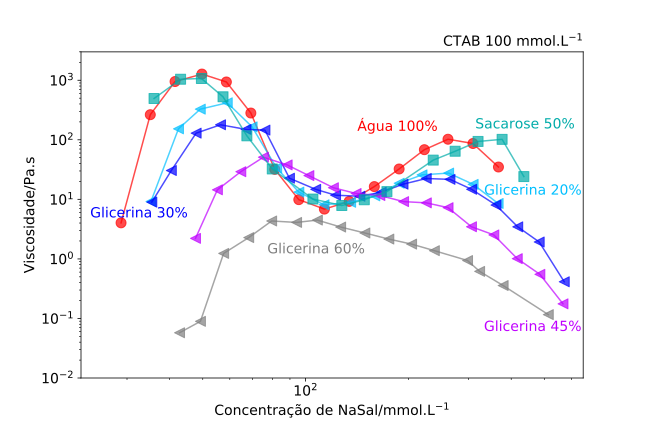
\includegraphics[width=0.7\textwidth]{imagens/reologia/RH_sacarose_glicerina}
				\caption{Viscosidade no repouso \(\eta_0\) em função da concentração de salicilato de sódio (NaSal) em várias concentrações dos aditivos glicerina e sacarose. 60\% de glicerina (V/V) e 50\% de sacarose (m/m) estão no ponto de equivalência do índice de refração.}
				\label{fig:rh_sacarose_glicerina}
			\end{figure} % todo: mencionar que curvas a laila mediu. Foram as de glicerina?
			
			Podemos observar que os dois picos de viscosidade observados em pequenas concentrações de glicerina, diminuem, e a região central permanece pouco afetada, como já havia sido descrito por Hoffmann. Porém, vemos que a adição de 50\% de sacarose praticamente não afetou a viscosidade das soluções, apesar da igualdade no índice de refração dessas soluções. Isso mostra que considerar somente o índice de refração não permite a previsão do comportamento dessas soluções, e isso motivou a realização de estudos posteriores.
			
			A figura \ref{fig:rh_13bd_dmso} mostra como os aditivos 1,3-butanodiol e dimetilsulfóxido afetam o perfil de viscosidade.
			
			\begin{figure}[h]
				\centering
				\includegraphics[width=0.7\textwidth]{imagens/reologia/RH_13BD_DMSO}
				\caption{Viscosidade no repouso \(\eta_0\) em função da concentração de salicilato de sódio (NaSal) em várias concentrações dos aditivos 1,3-butanodiol (1,3BD) e dimetilsulfóxido (DMSO). As concentrações de igualdade do índice de refração são 77\% (m/m) e 57\% (m/m), respectivamente}
				\label{fig:rh_13bd_dmso}
			\end{figure}
		
			O perfil de viscosidade dessas soluções foi muito mais afetado pelos aditivos do que era esperado observando-se somente o índice de refração, em especial o 1,3-butanodiol, onde 15\% (m/m) possui o mesmo efeito na viscosidade que 60\% de glicerina.
			
			A ureia possui o comportamento que mais difere dos outros aditivos, como mostra a figura \ref{fig:rh_ureia}.
			
			\begin{figure}[h]
				\centering
				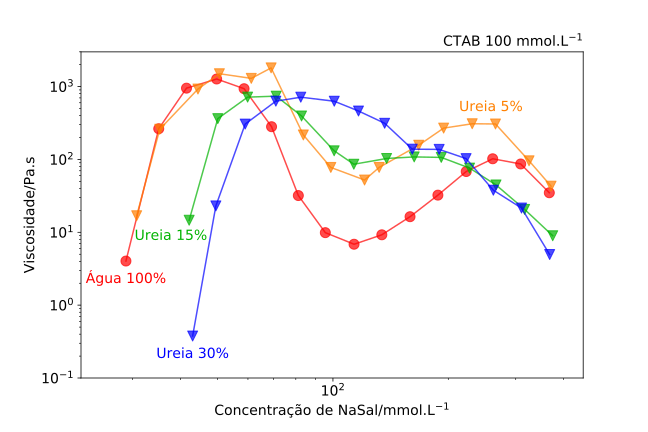
\includegraphics[width=0.7\textwidth]{imagens/reologia/RH_ureia}
				\caption{Viscosidade no repouso \(\eta_0\) em função da concentração de salicilato de sódio (NaSal) em várias concentrações de ureia. A concentração de igualdade de índice de refração é em torno de 55\%.}
				\label{fig:rh_ureia}
			\end{figure}

			Nesse caso, a viscosidade na região central aumentou, algo não observado nos outros cossolutos. Outro caso que possui um comportamento semelhante é o diagrama de orto-hidróxicinamato e \CTAB{} em pH 9. %todo: citar o artigo do OHCA
		
		\FloatBarrier
		
		\section{Efeito dos aditivos na calorimetria de micelas gigantes}
		
			A calorimetria de titulação isotérmica fornece informações sobre o quão favorável é a formação das micelas, através da concentração de formação de micelas gigantes, \cwlm. As figuras \ref{fig:itc_mg_glicerina} -- \ref{fig:itc_mg_ureia} mostram os perfis de formação de micelas gigantes para glicerina, sacarose, 1,3-butanodiol, dimetilsulfóxido e ureia.
		
			\begin{figure}[h]
				\centering
				\includegraphics[width=0.7\textwidth]{imagens/itc/ITC_MG_glic}
				\caption{Efeito da concentração de glicerina nas curvas de titulação de formação de micelas gigantes. A concentração de salicilato de sódio na cela de amostra é de 1,5\mM. A concentração do aditivo está em \% (V/V).}
				\label{fig:itc_mg_glicerina}
			\end{figure}  % todo: colocar a curva sem aditivo em todos. Trocar o 0% por uma curva preta.
			
			\begin{figure}[h]
				\centering
				\includegraphics[width=0.7\textwidth]{imagens/itc/ITC_MG_sac}
				\caption{Efeito da concentração de sacarose nas curvas de titulação de formação de micelas gigantes. A concentração de salicilato de sódio na cela de amostra é de 1,5\mM. A concentração do aditivo está em \% (m/m).}
				\label{fig:itc_mg_sacarose}
			\end{figure}
			
			As diferenças entre glicerina e sacarose, novamente, se evidenciaram. Da mesma maneira que na reologia, a presença de sacarose não afetou a formação de micelas gigantes. Já a glicerina teve um efeito deletério, aumentando significativamente a concentração necessária para o crescimento.
						
			\begin{figure}[h]
				\centering
				\includegraphics[width=0.7\textwidth]{imagens/itc/ITC_MG_13BD}
				\caption{Efeito da concentração de 1,3-butanodiol nas curvas de titulação de formação de micelas gigantes. A concentração de salicilato de sódio na cela de amostra é de 1,5\mM. A concentração do aditivo está em \% (m/m).}
				\label{fig:itc_mg_13bd}
			\end{figure}
			
			\begin{figure}[h]
				\centering
				\includegraphics[width=0.7\textwidth]{imagens/itc/ITC_MG_dmso}
				\caption{Efeito da concentração de dimetilsulfóxido nas curvas de titulação de formação de micelas gigantes. A concentração de salicilato de sódio na cela de amostra é de 1,5\mM. A concentração do aditivo está em \% (m/m).}
				\label{fig:itc_mg_dmso}
			\end{figure}  % todo: será que dá pra juntar os dois?

			1,3-BD e DMSO não se mostraram muito diferentes, apesar dos perfis reológicos serem bastante distintos, algo não totalmente inesperado, já que ambas as técnicas observam fenômenos diferentes. Isso indica que a queda de viscosidade com 1,3-BD não se deve à uma desestabilização micelar, o que levaria à uma diminuição na quantidade de micelas.

			\begin{figure}[h]
				\centering
				\includegraphics[width=0.7\textwidth]{imagens/itc/ITC_MG_ur}
				\caption{Efeito da concentração de ureia nas curvas de titulação de formação de micelas gigantes. A concentração de salicilato de sódio na cela de amostra é de 1,5\mM. A concentração do aditivo está em \% (m/m).}
				\label{fig:itc_mg_ureia}
			\end{figure}
		
			O comportamento da ureia seguiu o esperado, de acordo com a literatura, com um aumento de \cwlm{}. É interessante notar que o \DHwlm{} diminui com o aumento da concentração de ureia, o que sugere uma diminuição na adsorção de salicilato nas micelas. Em 35\% de ureia observa-se um perfil bastante diferente dos outros, porém nessa situação, ocorre a formação de um precipitado, cuja natureza será discutida na seção \ref{sec:cap_efeito_ureia}.
			
			Uma maneira de se resumir as curvas calorimétricas é através da concentração de formação de micelas gigantes (\cwlm) e a entalpia de micelização (\DHwlm). Dessa forma, podemos analisar o comportamento de todos os aditivos mais facilmente. A figura \ref{fig:cwlm_dhwlm_por_aditivo} resume isso, mostrando como essas propriedades variam com os aditivos, separadamente. A figura \ref{fig:cwlm_dhwlm_por_conc} mostra o mesmo, porém em função da concentração de aditivo.
			
			\begin{figure}[h]
				\begin{subfigure}[t]{0.5\textwidth}
					\centering
					\includegraphics[width=\textwidth]{imagens/itc/Cwlm_por_Aditivo}
					\caption{\cwlm{}}
					\label{fig:cwlm_por_aditivo}
				\end{subfigure}%
				\begin{subfigure}[t]{0.5\textwidth}
					\centering
					\includegraphics[width=\textwidth]{imagens/itc/DHwlm_por_Aditivo}
					\caption{\DHwlm{}}
					\label{fig:dhwlm_por_aditivo}
				\end{subfigure}
				\caption{\cwlm{} e \DHwlm{} em função dos aditivos e de sua concentração}
				\label{fig:cwlm_dhwlm_por_aditivo}
			\end{figure} 
		
			\begin{figure}[h]
				\begin{subfigure}[t]{0.5\textwidth}
					\centering
					\includegraphics[width=\textwidth]{imagens/itc/Cwlm_por_conc}
					\caption{\cwlm}
					\label{fig:cwlm_por_conc}
				\end{subfigure} %
				\begin{subfigure}[t]{0.5\textwidth}
					\centering
					\includegraphics[width=\textwidth]{imagens/itc/DHwlm_por_conc}
					\caption{\DHwlm}
					\label{fig:dhwlm_por_conc}
				\end{subfigure}
				
				\caption{\cmc{} e \DHmic{} em função da concentração de aditivo.}
				\label{fig:cwlm_dhwlm_por_conc}
			\end{figure}
		
		\FloatBarrier
		
		\section{Efeito dos aditivos na calorimetria de micelização}
		
		A calorimetria de formação de micelas gigantes possui uma complexidade maior devido à presença do salicilato. Para facilitar a interpretação, foram obtidas informações da formação de micelas esféricas, titulando-se \TTAB{} em água. As figuras \ref{fig:itc_glicerina} -- \ref{fig:itc_ureia} mostram as curvas de titulação para glicerina, sacarose, 1,3-butanodiol, dimetilsulfóxido e ureia.
					
%			\begin{figure}[h]
%				\centering
%				\includegraphics[width=0.7\textwidth]{imagens/itc/ITC_agua}
%				\caption{Titulação de \TTAB em água}
%				\label{fig:itc_agua}
%			\end{figure}
			
			\begin{figure}[h]
				\centering
				\includegraphics[width=0.7\textwidth]{imagens/itc/ITC_glic}
				\caption{Efeito da glicerina na titulação de \TTAB.}
				\label{fig:itc_glicerina}
			\end{figure}
		
			\begin{figure}[h]
				\centering
				\includegraphics[width=0.7\textwidth]{imagens/itc/ITC_sac}
				\caption{Efeito de sacarose na titulação de \TTAB}
				\label{fig:itc_sacarose}
			\end{figure}
			
			O efeito da glicerina na formação de micelas é semelhante ao efeito em micelas gigantes, exceto pelo aumento do \DHmic{}. Mais interessante, porém, é que sacarose levou à uma diminuição da \cmc{}. Isso levanta duas perguntas. Em primeiro lugar, qual é o mecanismo de estabilização micelar, e depois, porque esse mecanismo não afeta a formação de micelas gigantes?
			
			% todo: ref
			A literatura aponta que os grupos hidroxila pode interagir com a superfície micelar, diminuindo a repulsão entre as cabeças, estabilizando as micelas. Porém, nas micelas gigantes, o grupo carboxilato do salicilato se encontra nessa mesma região, então há uma competição entre esses dois grupos. Como o carboxilato é carregado, interage mais fortemente com as micelas e impede que a sacarose exerça sua influência estabilizadora. 
			
			\begin{figure}[h]
				\centering
				\includegraphics[width=0.7\textwidth]{imagens/itc/ITC_13BD}
				\caption{Efeito de 1,3-butanodiol na titulação de \TTAB}
				\label{fig:itc_13bd}
			\end{figure} 
		
			\begin{figure}[h]
				\centering
				\includegraphics[width=0.7\textwidth]{imagens/itc/ITC_dmso}
				\caption{Efeito de dimetilsulfóxido na titulação de \TTAB.}
				\label{fig:itc_dmso}
			\end{figure}
			
			Novamente, o 1,3-BD e DMSO mostraram possuir comportamentos semelhantes entre si, portanto o mecanismo que influencia ambas as micelas gigantes quanto esféricas deve ser semelhante.
			
			\begin{figure}[h]
				\centering
				\includegraphics[width=0.7\textwidth]{imagens/itc/ITC_ur}
				\caption{Efeito de ureia na titulação de \TTAB.}
				\label{fig:itc_ureia}
			\end{figure}
		
		A ureia influencia aumentando a \cmc{}, como esperado, porém não afeta muito o \DHmic{}. Logo, como não há \Sal{} para ser dessorvido das micelas, devido à alta constante dielétrica do meio, não há variações de \DHmic.
		
		As concentrações micelares críticas (\cmc) e entalpias de micelização (\DHmic) foram utilizadas para resumir as informações desta seção. A figura \ref{fig:cmc_dh_por_composto} mostra como as propriedades são afetadas pelos vários aditivos e suas concentrações, separadamente, e a figura \ref{fig:cmc_dh_por_conc} faz o mesmo, porém em função da concentração de aditivo.
		
		\begin{figure}[h]
			\begin{subfigure}[t]{0.5\textwidth}
				\centering
				\includegraphics[width=\textwidth]{imagens/itc/CMC_por_composto}
				\caption{\cmc}
				\label{fig:cmc_por_composto}
			\end{subfigure} %
			\begin{subfigure}[t]{0.5\textwidth}
				\centering
				\includegraphics[width=\textwidth]{imagens/itc/DH_por_composto}
				\caption{\DHmic}
				\label{fig:dh_por_composto}
			\end{subfigure}
		
			\caption{\cmc{} e \DHmic{} para os vários aditivos}
			\label{fig:cmc_dh_por_composto}
		\end{figure}

		\begin{figure}[h]
			\begin{subfigure}[t]{0.5\textwidth}
				\centering
				\includegraphics[width=\textwidth]{imagens/itc/ITC_cmc_adit}
				\caption{\cmc}
				\label{fig:cmc_por_conc}
			\end{subfigure} %
			\begin{subfigure}[t]{0.5\textwidth}
				\centering
				\includegraphics[width=\textwidth]{imagens/itc/ITC_DH_adit}
				\caption{\DHmic}
				\label{fig:dh_por_conc}
			\end{subfigure}
			
			\caption{\cmc{} e \DHmic{} em função da concentração de aditivo.}
			\label{fig:cmc_dh_por_conc}
		\end{figure}
	
		\FloatBarrier
		
	\chapter{Parâmetros a serem estudados}
		\section{Índice de refração}

		A figura \ref{fig:indice_refracao} mostrou como o índice de refração varia com a concentração de aditivo. Como os resultados reológicos evidenciaram, considerar somente o índice de refração não é uma maneira muito boa para explicar o comportamento reológico.
		
		Caso contrário, haveria um padrão notável num gráfico comparativo das concentrações e entalpias. Isso está evidenciado nas figuras \ref{fig:cmc_dh_por_n} e \ref{fig:cwlm_dhwlm_por_n}, onde não há um padrão geral observado para todos os aditivos.
		
		\begin{figure}[h]
			\begin{subfigure}[t]{0.5\textwidth}
				\centering
				\includegraphics[width=\textwidth]{imagens/itc/Cwlm_por_n}
				\caption{\cwlm}
				\label{fig:cwlm_por_n}
			\end{subfigure} %
			\begin{subfigure}[t]{0.5\textwidth}
				\centering
				\includegraphics[width=\textwidth]{imagens/itc/DHwlm_por_n}
				\caption{\DHwlm}
				\label{fig:dhwlm_por_n}
			\end{subfigure}
			
			\caption{\cwlm{} e \DHwlm{} em função do índice de refração.}
			\label{fig:cwlm_dhwlm_por_n}
		\end{figure}
		
		\begin{figure}[h]
			\begin{subfigure}[t]{0.5\textwidth}
				\centering
				\includegraphics[width=\textwidth]{imagens/itc/CMC_por_n}
				\caption{\cmc}
				\label{fig:cmc_por_n}
			\end{subfigure} %
			\begin{subfigure}[t]{0.5\textwidth}
				\centering
				\includegraphics[width=\textwidth]{imagens/itc/DH_por_n}
				\caption{\DHmic}
				\label{fig:dh_por_n}
			\end{subfigure}
			
			\caption{\cmc{} e \DHmic{} em função do índice de refração.}
			\label{fig:cmc_dh_por_n}
		\end{figure}

		Comparando-se as figuras \ref{fig:cwlm_dhwlm_por_n} e \ref{fig:cmc_dh_por_n}, pode-se observar que há uma correlação entre a formação de micelas gigantes e as concentrações críticas. Aparentemente há um grupo composto de 1,3BD, DMSO e ureia. Glicerina e sacarose se comportam bastante diferentemente, sendo que sacarose possui o comportamento mais diferenciado, não havendo mudança na \cwlm{} e uma diminuição da \cmc{}.
		
		Agrupamentos desse tipo não podem ser feitos com as entalpias, que parecem ter valores bastante variáveis. Porém, é necessário enfatizar que os valores de entalpia obtidos para a formação de micelas gigantes não são tão confiáveis quanto os de formação de micelas esféricas, já que estendeu-se a faixa de concentração de titulante, de modo a obter o perfil calorimétrico completo de todas as amostras. Isso reduz a precisão nos valores de entalpia iniciais. Esse problema possui menor relevância para \cwlm{}, que foi definida como sendo o ponto mínimo da curva, não uma subtração de duas regiões pré e pós-micelar. Apesar disso, o padrão observado para as mudanças de entalpia na presença de ureia podem ser explicadas pelo aumento da constante dielétrica do meio, como previamente mencionado.

		\FloatBarrier
		
		\section{Constante dielétrica}
		
		A constante dielétrica está relacionada ao grau de dissociação de espécies iônicas em solução. Quanto maior a constante, maior o grau de dissociação. Isso resulta, por exemplo, no aumento da \cmc{} pois há menos contraíons para reduzir a carga superficial micelar. A contribuição desse parâmetro já havia sido levantada em um estudo anterior. % todo: ref.
		A figura \ref{fig:cte_dieletrica} mostra como a constante dielétrica varia em função da concentração de aditivo. 
		
		\begin{figure}[h]
			\centering
			\includegraphics[width=0.7\textwidth]{imagens/propriedades/cte_dieletrica}
			\caption{Constante dielétrica em função da concentração de aditivo}
			\label{fig:cte_dieletrica}
		\end{figure}
	
		Da mesma maneira que o índice de refração, as concentrações micelares e entalpias dos processos serão comparados com a constante dielétrica do meio para tentar observar algum padrão.
		
		\begin{figure}[h]
			\begin{subfigure}[t]{0.5\textwidth}
				\centering
				\includegraphics[width=\textwidth]{imagens/itc/Cwlm_por_eps}
				\caption{\cwlm}
				\label{fig:cwlm_por_eps}
			\end{subfigure} %
			\begin{subfigure}[t]{0.5\textwidth}
				\centering
				\includegraphics[width=\textwidth]{imagens/itc/DHwlm_por_eps}
				\caption{\DHwlm}
				\label{fig:dhwlm_por_eps}
			\end{subfigure}
			
			\caption{\cwlm{} e \DHwlm{} em função da constante dielétrica \(\varepsilon\).}
			\label{fig:cwlm_dhwlm_por_eps}
		\end{figure}
		
		\begin{figure}[h]
			\begin{subfigure}[t]{0.5\textwidth}
				\centering
				\includegraphics[width=\textwidth]{imagens/itc/CMC_por_eps}
				\caption{\cmc}
				\label{fig:cmc_por_eps}
			\end{subfigure} %
			\begin{subfigure}[t]{0.5\textwidth}
				\centering
				\includegraphics[width=\textwidth]{imagens/itc/DH_por_eps}
				\caption{\DHmic}
				\label{fig:dh_por_eps}
			\end{subfigure}
			
			\caption{\cmc{} e \DHmic{} em função da constante dielétrica \(\varepsilon\).}
			\label{fig:cmc_dh_por_eps}
		\end{figure}
		
		\FloatBarrier
		\section{Parâmetro de Gordon}
		\section{Interação dos aditivos com a superfície micelar}
		\section{Decomposição em propriedades fundamentais}
	\chapter{Correlações entre os parâmetros e as propriedades}
		\section{Reologia}
		\section{Calorimetria}

\chapter{Efeito da ureia}
	\section{Motivação}
	A ureia demonstrou um comportamento que divergiu bastante dos outros aditivos. Por esse motivo, ela será estudada um pouco mais profundamente. Porém, a ação do salicilato de sódio não receberá muito enfoque, para simplificar o sistema. Portanto, foi estudado principalmente o efeito da ureia em soluções de CTAB, TTAB e DTAB, com concentrações diferentes de ureia e de surfactante.
	
	Ocorre a formação de um precipitado esbranquiçado em soluções de surfactante em concentrações maiores que 35\% de ureia. Isso ocorre a temperatura ambiente. Quando a solução é aquecida acima de cerca de 35ºC, ela se torna transparente. Esse comportamento foi estudado, variando-se o surfactante, sua concentração, e a concentração de ureia. Desses sistemas, foram estudadas as características térmicas, a estrutura da mesofase, e a reologia da fase esbranquiçada.
	
	\section{Calorimetria diferencial de varredura (DSC)}

		Foram preparadas soluções de ureia, em várias concentrações, com três surfactantes (CTAB, TTAB e DTAB), em três concentrações. Os termogramas resultantes foram organizados em figuras de modo a facilitar comparações. A tabela \ref{tab:refs_DSC} lista as comparações realizadas e em quais figuras estão.
        
        \begin{table}[H]
            \IBGEtab{%
                \caption{Comparações de termogramas de amostras de surfactante (concentração em \mM)e ureia (\% m/m), e suas respectivas figuras}
                \label{tab:refs_DSC}
                }%
                {%
                \begin{tabular}{l c c}
                    \toprule
        			%\centering
        			Surf. \mM     & \% Ureia		& Figura 			\\
        			\midrule
        			CTAB 100	  & 38--45			& \ref{fig:DSC_CTAB_UR38-45}	\\
        			CTAB 100, 200, 300	& 45, 40	& \ref{fig:DSC_CTAB_UR40-45}	\\
        			TTAB 100, 200, 300	& 45, 40	& \ref{fig:DSC_TTAB_UR_40-45}	\\
        			DTAB 100, 200, 300	& 45, 40	& \ref{fig:DSC_DTAB_UR_40-45}	\\
        			CTAB, TTAB, DTAB 100	& 45	& \ref{fig:DSC_Surf_100mm_45p}	\\
        			CTAB, TTAB, DTAB 200	& 45	& \ref{fig:DSC_Surf_200mm_45p}	\\
        			CTAB, TTAB, DTAB 300	& 45	& \ref{fig:DSC_Surf_300mm_45p}	\\
        			\midrule
        			CTAB 100 NaSal 60	& 35, 40, 45	& \ref{fig:DSC_NaSal60}		\\
        			CTAB 100 NaSal 100	& 35, 40, 45	& \ref{fig:DSC_NaSal100}	\\
        			CTAB 100 NaSal 250	& 35, 40, 45	& \ref{fig:DSC_NaSal250}	\\
        			CTAB 100 NaSal 60, 100, 250 & 35 	& \ref{fig:DSC_NaSal_Ur35}  \\
        			CTAB 100 NaSal 60, 100, 250 & 40	& \ref{fig:DSC_NaSal_Ur40}  \\
        			CTAB 100 NaSal 60, 100, 250	& 45	& \ref{fig:DSC_NaSal_Ur45}  \\
        			\bottomrule
                \end{tabular}%
                }{}
        \end{table}
		
		% todo: cortar o número de figuras para diminuir repetição, adicionar outros gráficos mostrando como os parâmetros são afetados
		% todo: tirar CTAB 400 mM? Ele foje em muitos casos do esperado. Como explicar?
		
		\begin{figure}[H]
			\centering
			\includegraphics[width=0.75\textwidth]{./imagens/dsc/CTAB_porc_ur}
			\caption{Termogramas de soluções de CTAB 100 \mM{} em concentrações crescentes de ureia, de 38\% m/m a 45\% m/m}
			\label{fig:DSC_CTAB_UR38-45}
		\end{figure}
		
		\begin{figure}[H]
			\begin{subfigure}[t]{0.45\textwidth}
				\centering
				\includegraphics[width=\textwidth]{./imagens/dsc/CTAB_45p}
				\caption{45\% de ureia}
				\label{fig:DSC_CTAB_UR45}
			\end{subfigure} \qquad %
			\begin{subfigure}[t]{0.45\textwidth}
				\centering
				\includegraphics[width=\textwidth]{./imagens/dsc/CTAB_40p}
				\caption{40\% de ureia}
				\label{fig:DSC_CTAB_UR40}
			\end{subfigure}
			\caption{Termogramas de CTAB 100, 200 e 300 \mM{} em soluções em 45\% (\ref{fig:DSC_CTAB_UR45}) e 40\% (\ref{fig:DSC_CTAB_UR40})}
			\label{fig:DSC_CTAB_UR40-45}
		\end{figure}
	
		\begin{figure}[H]
			\centering
			\begin{subfigure}[t]{0.45\textwidth}
				\includegraphics[width=\textwidth]{./imagens/dsc/TTAB_45p}
				\caption{45\% de ureia}
				\label{fig:DSC_TTAB_UR45}
			\end{subfigure} \qquad %
			\begin{subfigure}[t]{0.45\textwidth}
				\includegraphics[width=\textwidth]{./imagens/dsc/TTAB_40p}
				\caption{40\% de ureia}
				\label{fig:DSC_TTAB_UR40}
			\end{subfigure}
			\caption{Termogramas de soluções de TTAB 100, 200 e 300 \mM{}, em 45\% (\ref{fig:DSC_TTAB_UR45}) e 40\% (\ref{fig:DSC_TTAB_UR40}) de ureia}
			\label{fig:DSC_TTAB_UR_40-45}
		\end{figure}
		
		\begin{figure}[H]
			\centering
			\begin{subfigure}[t]{0.45\textwidth}
				\includegraphics[width=\textwidth]{./imagens/dsc/DTAB_45p}
				\caption{45\% de ureia}
				\label{fig:DSC_DTAB_UR45}
			\end{subfigure} \qquad %
			\begin{subfigure}[t]{0.45\textwidth}
				\includegraphics[width=\textwidth]{./imagens/dsc/DTAB_40p}
				\caption{40\% de ureia}
				\label{fig:DSC_DTAB_UR40}
			\end{subfigure}
			\caption{Termogramas de soluções de DTAB 100, 200 e 300 \mM{}, em 45\% (\ref{fig:DSC_DTAB_UR45}) e 40\% (\ref{fig:DSC_DTAB_UR40}) de ureia}
			\label{fig:DSC_DTAB_UR_40-45}
		\end{figure}
		
		
		% todo: verificar se a notação (C|T|D) é boa
		\begin{figure}[H]
			\centering
			\includegraphics[width=0.60\textwidth]{./imagens/dsc/Surf_100mm_45p}
			\caption{Termogramas de soluções de (C|T|D)TAB 100 \mM{}, em 45\% de ureia}
			\label{fig:DSC_Surf_100mm_45p}
		\end{figure}
	
		\begin{figure}[H]
			\centering
			\includegraphics[width=0.60\textwidth]{./imagens/dsc/Surf_200mm_45p}
			\caption{Termogramas de soluções de (C|T|D)TAB 200 \mM{}, em 45\% de ureia}
			\label{fig:DSC_Surf_200mm_45p}
		\end{figure}
	
		\begin{figure}[H]
			\centering
			\includegraphics[width=0.60\textwidth]{./imagens/dsc/Surf_300mm_45p}
			\caption{Termogramas de soluções de (C|T|D)TAB 300 \mM{}, em 45\% de ureia}
			\label{fig:DSC_Surf_300mm_45p}
		\end{figure}
	
		\begin{figure}[H]
			\centering
			\includegraphics[width=0.60\textwidth]{./imagens/dsc/NaSal60}
			\caption{Termogramas de soluções de NaSal 60\mM{} e CTAB 100 \mM{}, em 35\%, 40\% e 45\% (m/m) de ureia}
			\label{fig:DSC_NaSal60}
		\end{figure}
	
		\begin{figure}[H]
			\centering
			\includegraphics[width=0.60\textwidth]{./imagens/dsc/NaSal100}
			\caption{Termogramas de soluções de NaSal 100\mM{} e CTAB 100 \mM{}, em 35\%, 40\% e 45\% (m/m) de ureia}
			\label{fig:DSC_NaSal100}
		\end{figure}

		\begin{figure}[H]
			\centering
			\includegraphics[width=0.60\textwidth]{./imagens/dsc/NaSal250}
			\caption{Termogramas de soluções de NaSal 250\mM{} e CTAB 100 \mM{}, em 35\%, 40\% e 45\% (m/m) de ureia}
			\label{fig:DSC_NaSal250}
		\end{figure}
	
		\begin{figure}[H]
			\centering
			\includegraphics[width=0.60\textwidth]{./imagens/dsc/NaSal35}
			\caption{Termogramas de soluções de NaSal 60, 100 e 250\mM{} e CTAB 100 \mM{}, em 35\% (m/m) de ureia}
			\label{fig:DSC_NaSal_Ur35}
		\end{figure}
	
		\begin{figure}[H]
			\centering
			\includegraphics[width=0.60\textwidth]{./imagens/dsc/NaSal40}
			\caption{Termogramas de soluções de NaSal 60, 100 e 250\mM{} e CTAB 100 \mM{}, em 40\% (m/m) de ureia}
			\label{fig:DSC_NaSal_Ur40}
		\end{figure}

		\begin{figure}[H]
			\centering
			\includegraphics[width=0.60\textwidth]{./imagens/dsc/NaSal45}
			\caption{Termogramas de soluções de NaSal 60, 100 e 250\mM{} e CTAB 100 \mM{}, em 45\% (m/m) de ureia}
			\label{fig:DSC_NaSal_Ur45}
		\end{figure}

			
		% (Figs. \ref{fig:DSC_CTAB_UR38-45}, \ref{fig:DSC_CTAB_UR40-45}, \ref{fig:DSC_TTAB_UR_40-45}, \ref{fig:DSC_DTAB_UR_40-45}, \ref{fig:DSC_NaSal60}, \ref{fig:DSC_NaSal100}, \ref{fig:DSC_NaSal250})
		Qualitativamente, podemos observar que com o aumento de concentração de ureia, a temperatura de transição também aumenta. Além disso, vemos que CTAB e TTAB possuem temperaturas semelhantes de transição, maiores que DTAB (Figs. \ref{fig:DSC_Surf_100mm_45p}, \ref{fig:DSC_Surf_200mm_45p}, \ref{fig:DSC_Surf_300mm_45p}).
		
		% todo: será que dá pra fazer alguma análise estatística aqui? Ou plotar mais gráficos?
		
		As áreas de transição, e a largura dos picos são, também, proporcionais à concentração de surfactante utilizado. Quanto maior a concentração, maior 
		
		 A adição de NaSal causa uma diminuição na temperatura de transição, especialmente visível em 250\mM{} de NaSal. As tabelas \ref{tab:DSC_temp_areas} e \ref{tab:DSC_temp_areas_NaSal} mostram as temperaturas de transição no aquecimento e resfriamento, obtidas pelo valor do máximo do pico, as áreas de transição e as larguras a meia altura dos picos 

        \begin{table}[H]
            \IBGEtab%
            {\caption{Temperaturas de transição ($T$/°C), áreas de transição por mol de surfactante ($A$/$J.mol^{-1}$) e largura a meia altura dos picos de transição ($L$/°C) dos ciclos de aquecimento (\emph{aq}) e resfriamento (\emph{res}) para três surfactantes (Surf.), CTAB, TTAB, DTAB, cujas concentrações estão em \mM, em várias concentrações \% (m/m) de ureia}
            \label{tab:DSC_temp_areas}}%
            {\begin{tabular}{ccccccccc}
                \toprule
    			\% Ur. & Surf. & $C_{surf}$ &
    			$T_{aq}$ & $T_{res}$ & $A_{aq}$ & $A_{res}$ & $L_{aq}$ & $L_{res}$\\
    			\midrule
    			38 & CTAB & 100 & 30,5 & 19,3 & 2,67 & 2,68 & 5,6 &	3,0\\
    			39 & CTAB & 100 & 32,5 & 25,2 & 2,28 & 2,30 & 6,4 &	2,4\\
    			40 & CTAB & 100 & 33,3 & 25,1 & 4,73 & 4,41 & 5,6 &	3,0\\
    			41 & CTAB & 100 & 34,1 & 27,2 & 1,74 & 1,77 & 5,3 &	1,6\\
    			42 & CTAB & 100 & 37,5 & 29,6 & 2,71 & 2,75 & 6,0 &	1,9\\
    			43 & CTAB & 100 & 38,7 & 31,1 & 2,10 & 2,10 & 5,4 &	1,8\\
    			44 & CTAB & 100 & 40,2 & 34,6 & 1,86 & 1,85 & 4,9 &	1,6\\
    			45 & CTAB & 100 & 41,0 & 34,6 & 2,04 & 2,02 & 4,6 &	1,5\\
    			\midrule
    			40 & CTAB & 200 & 31,6 & 23,6 & 4,75 & 4,81 & 6,4 &	2,4\\
    			45 & CTAB & 200 & 41,6 & 34,9 & 1,72 & 1,92 & 10,3 & 3,5\\
    			40 & CTAB & 300 & 31,7 & 24,8 & 4,84 & 4,79 & 5,3 &	1,6\\
    			45 & CTAB & 300 & 41,4 & 32,8 & 2,40 & 2,44 & 15,4 & 5,8\\
    			35 & CTAB & 400 & 21,9 & 21,9 & 2,93 & 1,52 & 24,0 & 12,3\\
    			40 & CTAB & 400 & 36,4 & 26,5 & 2,99 & 1,78 & 23,3 & 7,4\\
    			45 & CTAB & 400 & 43,4 & 33,6 & 3,79 & 3,74 & 21,7 & 7,4\\
    			\midrule
    			40 & DTAB & 100 & 26,7 & 22,5 & 1,77 & 1,71 & 6,0 & 1,9\\
    			45 & DTAB & 100 & 33,0 & 30,1 & 1,39 & 1,48 & 2,5 & 1,1\\
    			40 & DTAB & 200 & 27,4 & 22,8 & 2,34 & 2,27 & 5,4 &	1,8\\
    			45 & DTAB & 200 & 33,4 & 30,0 & 1,83 & 1,88 & 6,3 &	2,8\\
    			40 & DTAB & 300 & 26,2 & 21,5 & 1,87 & 1,93 & 4,9 &	1,6\\
    			45 & DTAB & 300 & 33,5 & 29,8 & 2,04 & 2,13 & 10,6 & 3,7\\
    			\midrule
    			40 & TTAB & 100 & 31,9 & 26,4 & 4,94 & 5,04 & 4,6 &	1,5\\
    			45 & TTAB & 100 & 37,8 & 34,7 & 2,25 & 2,29 & 4,7 &	1,6\\
    			40 & TTAB & 200 & 31,9 & 25,3 & 3,94 & 4,00 & 10,3 & 3,5\\
    			45 & TTAB & 200 & 37,4 & 33,8 & 1,85 & 1,90 & 8,8 &	2,6\\
    			40 & TTAB & 300 & 29,8 & 26,5 & 4,81 & 4,61 & 15,4 & 5,8\\
    			45 & TTAB & 300 & 37,8 & 33,2 & 2,03 & 2,06 & 14,0 & 4,1\\
                \bottomrule
                \end{tabular}}%
            {}
        \end{table}
        
      \begin{table}[H]
          \IBGEtab%
          {\caption{Temperaturas de transição ($T$/°C), áreas de transição por mol de surfactante ($A$/$J.mol^{-1}$) e largura a meia altura dos picos de transição ($L$/°C) dos ciclos de aquecimento (\emph{aq}) e resfriamento (\emph{res}) para CTAB com NaSal, cujas concentrações estão em \mM, em três concentrações \% (m/m) de ureia}
          \label{tab:DSC_temp_areas_NaSal}}%
            {\begin{tabular}{cccccccccc}
                \toprule
                \% Ur. & Surf. & $C_{surf}$ & $C_{NaSal}$ &
                $T_{aq}$ & $T_{res}$ & $A_{aq}$ & $A_{res}$ & $L_{aq}$ & $L_{res}$\\
       			\midrule
       			35 & CTAB & 100 & 60 & 22,0 & 14,6 & 5,07 & 3,48 & - & -\\
       			40 & CTAB & 100 & 60 & 27,6 & 22,0 & 6,67 & 6,18 & - & -\\
       			45 & CTAB & 100 & 60 & 42,0 & 23,5 & 5,66 & 4,06 & 15,0 & 3,0\\
       			35 & CTAB & 100 & 100 & 20,7 & - & 5,00 & - & 10,9 & -\\
       			40 & CTAB & 100 & 100 & 27,1 & 22,9 & 7,03 & 5,82 & 15,3 &	9,1\\
       			45 & CTAB & 100 & 100 & 29,9 & 26,0 & 5,51 & 4,87 & 11,0 &	8,5\\
       			35 & CTAB & 100 & 250 & 22,8 & 12,7 & 6,05 & 2,98 & 8,5 &	8,7\\
       			40 & CTAB & 100 & 250 & 23,3 & 11,8 & 4,55 & 2,60 & 7,1 &	7,5\\
       			45 & CTAB & 100 & 250 & 29,1 & 27,0 & 9,99 & 5,93 & 12,3 &	6,9\\
       			\bottomrule
            \end{tabular}}%
                {}
            \end{table}

		
	\section{SAXS}
	\section{DLS}
	\section{Reologia do sólido}
	\section{Entalpia de interação de ureia com surfactante}
	
\part{Cinética de crescimento}
	\chapter{SAXS resolvido no tempo}
	\chapter{Fluorescência resolvida no tempo}
\part{Contribuições para outros projetos}

	\chapter{Breve descrição sobre o projeto de fibrose cística}

	Durante a execução do projeto de doutorado, foi estabelecida uma parceria com uma aluna de doutorado da Faculdade de Ciências Médicas na Unicamp, Carla Cristina S. Gomez, através do Professor Francisco Benedito Pessine, do Instituto de Química da Unicamp, para a análise de amostras de muco de pacientes com fibrose cística. Nesta seção, uma pequena descrição sobre o projeto será apresentada, a contribuição do aluno será realçada, e os resultados do projeto serão mencionados.
	
	Uma alteração genética no gene que controla a produção da proteína CFTR (Cystic Fibrosis Transmembrane Conductante Regulator), pode causar uma disfunção do transporte de íons cloreto. Essa alteração genética resulta numa série de problemas corporais, e essa doença é conhecida de forma geral como fibrose cística. % todo: procurar a incidência dessa doença
	
	Além de afetar o transporte de cloreto, recentemente foi notado que a secreção de bicarbonato na superfície das vias aéreas é bloqueada. Isso resulta em mais íons cálcio livres e uma capacidade tamponante enfraquecida. As mucinas, componentes do muco, secretadas para lubrificar o epitélio e servir como barreira contra patógenos, são afetadas pelo excesso de Ca2+ e pelo pH baixo. Ocorre sua desidratação, tornando o muco mais espesso, comprometendo sua função de lubrificação. Além disso, o pH baixo leva a uma promoção do crescimento de bactérias, acarretando na formação de biofilme e alteração da resposta imunológica.
	
	A principal causa de mortalidade da fibrose cística é a deterioração da função pulmonar através da inflamação e infecção das vias aéreas. Logo, se os sintomas causados pela fibrose cística no pulmão forem eficientemente combatidos, haveria uma melhoria tanto na qualidade quanto na expectativa de vida dos pacientes. Poucos estudos testaram o efeito do bicarbonato nas vias aéreas, porém observou-se que o bicarbonato possui efeitos positivos. Esses são, redução da viscosidade do muco, melhorando a lubrificação, diminuição das feridas causadas pela tosse, e remoção de detritos dos pulmões, além de aumento o pH, diminuindo a proliferação bacteriana. Logo, um estudo para verificar se essas alterações no muco pela inalação de bicarbonato afetariam positivamente os pacientes, e se a inalação em si é tolerável, é importante. Este é o primeiro estudo \emph{in vivo} dessa natureza.
	
	Uma série de 19 voluntários com fibrose cística participaram do estudo, porém 7 descontinuaram. Eles foram dosados com soluções 4,2\% e 8,4\% de NaHCO3 diluído em água destilada, por inalação, e depois de duas triagens, recebiam o produto para realizar a inalação domiciliarmente. Após isso, retornavam ao centro de pesquisa para escarrar, a cada meia hora, e o muco era coletado e depois analisado. Primeiramente o pH era medido, e depois as amostras eram enviadas para serem analisadas no instituto de química. Os parâmetros das análises foram determinados pelo autor da tese, e aproximadamente metade das amostras foram analisadas pelo mesmo (cerca de 250). As amostras restantes foram analisadas pela aluna Carla Gomez. Após isso, os resultados foram tratados, e o processo de tratamento de dados será descrito nesta parte.


	\chapter{Contribuições ao projeto}
	
	Nesse projeto, foram analisados tanto curvas de fluxo, como a reologia oscilatória do muco. Utilizou-se tanto o reômetro Haake RheoStress1 quanto o Haake Mars III, ambos da Thermo Scientific, para as análises. Para o tratamento de dados, foi utilizado a linguagem Python, que permite resultados consistentes e de melhor qualidade, se comparados com o ajuste manual.
	
		\section{Determinação dos parâmetros de análise}
		
		Foram analisadas algumas amostras inicialmente para se determinar as faixas de varredura para os estudos reológicos. Primeiramente, a faixa linear de tensão foi determinada com uma varredura de 0,01 Pa a 0,75 Pa, a 1 Hz. Após isso, a varredura oscilatória de frequência foi medida, geralmente com tensões de 0,5 Pa, entre 0,1 Hz a 5 Hz. As curvas de fluxo foram medidas entre 0,01 a 1 s\menosUm.
	
		\section{Criação de um software para tratamento de curvas de fluxo}
		\label{sec:apn_tratamento_CF}
		Para o tratamento de dados de curva de fluxo, foi criado um programa que permite o usuário aplicar três modelos mais complexos e um modelo simplificado para a obtenção de valores de viscosidade no repouso. Todas as amostras de muco, sem exceção, demonstraram ser pseudoplásticas, então não foram colocados mais modelos. A seguir, será mostrado os modelos utilizados e seções da lógica do programa, pois o código fonte inteiro é longo demais para ser incluído aqui (aproximadamente 1000 linhas).
		
			\subsection{Modelos de curvas de fluxo pseudoplásticas}
		\label{sec:modelagem_curva_fluxo}
		Foram implementados os modelos de \emph{Carreau-Yasuda} (Eq \ref{eqn:AP_CarreauYasuda}), \emph{Carreau} (Eq. \ref{eqn:AP_Carreau}), \emph{Cross} (Eq. \ref{eqn:AP_Cross}) e \emph{linear}, de maior para menor complexidade, respectivamente. Os modelos correlacionam a taxa de cisalhamento (\(\dot{\gamma}\), variável independente) à viscosidade (\(\eta\), variável dependente) utilizando alguns parâmetros.
		
		\begin{equation}
		\eta = \eta_{\infty} + \frac{\eta_0 - \eta_{\infty}}{\left[  1 + \left(  \dfrac{\dot{\gamma}}{\dot{\gamma}_b}  \right)^{a}  \right]^{\frac{ \left(  n - 1  \right) }{a}}}
		\label{eqn:AP_CarreauYasuda}
		\end{equation}
		
		\begin{equation}
		\eta = \eta_{\infty} + \frac{\eta_0 - \eta_{\infty}}{\left[  1 + \left(  \dfrac{\dot{\gamma}}{\dot{\gamma}_b}  \right)^{2}  \right]^{\frac{n}{2}}}
		\label{eqn:AP_Carreau}
		\end{equation}
		
		\begin{equation}
		\eta = \eta_{\infty} + \frac{\eta_0 - \eta_{\infty}}{1 + \left(  \dfrac{\dot{\gamma}}{\dot{\gamma}_b}  \right)^{n}}
		\label{eqn:AP_Cross}
		\end{equation}
		
		O modelo linear considera somente valores de viscosidade em \(\dot{\gamma}\) próximos de zero, ou seja, \(\eta = \eta_0 + 0 \times \dot{\gamma}\).
		
		Os parâmetros possuem os seguintes significados:
		
		\begin{table}[H]
			\IBGEtab{%
				\caption{Parâmetros dos modelos de fluidos pseudoplásticos}
				\label{tab:params_pseudoplasticos}
			}%
			{%
				\begin{tabular}{c c p{9cm}}
					\toprule
					    Parâmetro      & Unidade   & Significado                                                       \\ \midrule
					    \(\eta_0\)     & Pa.s      & Viscosidade no repouso*                                           \\
					\(\eta_{\infty}\)  & Pa.s      & Viscosidade no infinito                                           \\
					      \(n\)        & --        & Inclinação da região de decaimento de viscosidade                 \\
					\(\dot{\gamma}_b\) & s\menosUm & \(\dot{\gamma}\) de início da região de decaimento de viscosidade \\ \midrule
					      \(a\)        & --        & Afeta tanto a inclinação quanto o ponto de inflexão               \\ \bottomrule
				\end{tabular}%
			}{}
		\end{table}
		% todo: pensar em colocar os gráficos mostrando como esses parâmetros afetam as curvas
		% todo: pensar um pouco mais sobre o Carreau-Yasuda e como que o a deve se comportar
		
		A Fig. \ref{fig:reologia_modelos} exemplifica os modelos de Carreau e Cross e como os parâmetros afetam o formato das curvas. Note que a escala dos eixos é logarítmica. Vemos que, essencialmente, ambas as curvas possuem formatos muito semelhantes, com os parâmetros escolhidos. A escolha de um modelo depende da qualidade dos dados e do desejo do experimentalista. Observando-se como os modelos variam com os parâmetros, nota-se que a queda de viscosidade do modelo de Carreau é menos abrupta que no modelo de Cross e se assemelha mais aos dados estudados, então esse modelo foi mais utilizado.
		
		\begin{figure}[H]
			\begin{subfigure}[t]{0.45\textwidth}
				\centering
				\includegraphics[width=\textwidth]{./imagens/reologia/Carreau}
				\caption{Modelo de Carreau}
				\label{fig:reologia_modelo_carreau}
			\end{subfigure} \qquad %
			\begin{subfigure}[t]{0.45\textwidth}
				\centering
				\includegraphics[width=\textwidth]{./imagens/reologia/Cross}
				\caption{Modelo de Cross}
				\label{fig:reologia_modelo_cross}
			\end{subfigure}
			\caption{Exemplos de curvas de fluxo descritas pelos modelos de Carreau e Cross, com os parâmetros utilizados.}
			\label{fig:reologia_modelos}
		\end{figure}
		
		De maior interesse para os estudos neste trabalho é a viscosidade no repouso, \(\eta_0\), e portanto esse é o foco do programa. Porém, o ajuste indiscriminado de um modelo a um dado experimental é problemático caso a qualidade do dado não seja boa, seja pela própria característica da amostra, ou pela sensibilidade do equipamento. Por exemplo, é frequente que apareçam artefatos de medida em baixos valores de \(\dot{\gamma}\), resultando ou num decréscimo ou acréscimo gradual de \(\eta\). Além disso, é possível que não seja observada a região descrita por \(\eta_{\infty}\), em altos valores de \(\dot{\gamma}\), o que atribui grande incerteza na determinação desse parâmetro. Dessa forma, é necessário que uma região das curvas seja escolhida para que o ajuste seja bem sucedido e informativo, o que representa a maior dificuldade nesse tipo de análise, devido à certa subjetividade no critério de escolha da região de ajuste.
		
		Por essa razão, e outras, como velocidade de análise, foi escrito o método de ajuste. O método consiste em realizar ajustes sucessivos, entre um ponto inicial \(P_i\) até um ponto final \(P_f\), e depois comparar os resultados dos ajustes para escolher um deles. Podem ser comparados, por exemplo, os parâmetros \(R^2\), \(\chi^2\) ou \(\chi_{red}^2\). Escolhido o melhor ajuste, observando-se, por exemplo, a maior proximidade de \(R^2\) a 1 ou de \(\chi^2\) a 0, tomando cuidado para não escolher uma faixa muito estreita de pontos, os resultados são graficados, gravados num arquivo de texto e passa-se para o próximo dado experimental.
		
		A listagem \ref{lst:exemplo_curva_de_fluxo} mostra duas seções do código completo do programa, uma mostrando o ciclo de ajuste utilizando o ajuste linear e \texttt{curve\_fit} e outro que realiza um ajuste não-linear utilizando o modelo de Carreau e \emph{lmfit}.
		
		\begin{listing}[H]
			\inputminted{python}{./python/curva_de_fluxo.py}
			\caption{Seções do código mostrando o método de ajuste}  % todo: encontrar um nome melhor
			\label{lst:exemplo_curva_de_fluxo}
		\end{listing}
		
		Essas funções estão dentro de uma classe chamada \texttt{Fitter}. Para utilizar essa classe em outros códigos, é necessário inicializar uma instância da classe \texttt{Settings} e depois inicializar uma instância da classe \texttt{Fitter} utilizando as configurações da classe \texttt{Settings}. Caso não haja um arquivo \texttt{settings.dat} na pasta, um arquivo com valores padrão será criado. Após isso, é possível tanto editar o arquivo \texttt{settings.dat} quando utilizar as funções \texttt{print\_settings, edit\_settings} do objeto \texttt{Settings}. Ao criar um objeto \emph{Fitter}, por padrão os ajustes configurados já são realizados e os resultados são mostrados na tela. Caso se deseja criar um gráfico mostrando o resultado dos ajustes, pode-se chamar a função \texttt{plot\_error\_graphs()}. 
		
		A listagem \ref{lst:exemplo_fitter} mostra como o programa pode ser utilizado por outros scripts, e o resultado do ajuste se encontra na Fig. \ref{fig:reologia_dado-exemplo}
		
		\begin{listing}[H]
			\inputminted{python}{./python/uso_fitter.py}
			\caption{Exemplo de como utilizar a ferramenta de ajuste não linear}  % todo: encontrar um nome melhor
			\label{lst:exemplo_fitter}
		\end{listing}
		
		\begin{figure}[H]
			\centering
			\includegraphics[width=\textwidth]{imagens/reologia/Dado-exemplo}
			\caption{Figura resultante do ajuste não linear de Carreau e ajuste linear gerada pela função \texttt{plot\_error\_graphs()}. As barras de erro são oriundas da propagação de erro dos parâmetros e os números em vermelho indicam os pontos iniciais e finais considerados em cada ajuste.}
			\label{fig:reologia_dado-exemplo}
		\end{figure}
		
		Note que no dado utilizado, não há muitos problemas de desvio da curva, então os ajustes foram bem comportados. Os exemplos das figuras \ref{fig:reologia_dado-problemadescida} e \ref{fig:reologia_dado-problemasubida} mostram problemas reais na região de baixos valores de \(\dot{\gamma}\).
		
		\begin{figure}
			\centering
			\includegraphics[width=\textwidth]{imagens/reologia/Dado-ProblemaDescida}
			\caption{Exemplo dos ajustes não-linear e linear de um dado real que possui uma queda nos valores de \(\eta\) em baixas \(\dot{\gamma}\)}
			\label{fig:reologia_dado-problemadescida}
		\end{figure}
		
		\begin{figure}
			\centering
			\includegraphics[width=\textwidth]{imagens/reologia/Dado-ProblemaSubida}
			\caption{Exemplo dos ajustes não-linear e linear de um dado real que possui um aumento nos valores de \(\eta\) em baixas \(\dot{\gamma}\)}
			\label{fig:reologia_dado-problemasubida}
		\end{figure}
		
		O tempo de execução e de plotagem para cada experimento está na faixa de um segundo, o que é muito mais rápido do que realizar o ajuste manualmente em uma ferramenta como o Origin ou Excel, então é algo ideal para o tratamento de um grande volume de dados.
		

		\section{Método de ajuste para reologia oscilatória de muco}
		
		As amostras de muco não seguiram modelos de reologia parecidos aos apresentados neste trabalho, como o modelo de Maxwell. Portanto, foi necessário desenvolver uma nova abordagem para analisar as amostras. Plotando-se todos os dados obtidos, observou-se que G' estava sempre acima de G'' e, na escala logarítmica, as duas curvas eram praticamente paralelas e ligeiramente inclinadas positivamente. Em alguns casos, a inclinação aumentava em frequências maiores e, frequentemente, havia uma oscilação de G' e G'' sem significado físico nessa região. A taxa de aumento era consistente com uma exponencial. Visto isso, foi desenvolvido um script que realiza o seguinte:
		
		\begin{enumerate}
			\item Obter a região de frequência confiável de G' e de G'' para o modelo linear e exponencial. Isso é feito realizando-se ajustes gradativos, do primeiro ponto até um ponto \emph{n}, armazenando os ajustes e depois escolhendo o ajuste com maior número de pontos onde \(R^2 > 0{,}9\). Caso não exista ajuste seguindo esse critério, escolhe-se um novo critério com \(R^2 > 0,85\). Caso não exista ajuste que obedeça isso mesmo assim, é escolhido o ajuste com o maior número de pontos. 
			\item Os parâmetros dos ajustes que passaram pelo filtro de \(R^2\) são gravados em um arquivo \texttt{csv}. Além disso, são gravados a média dos valores de G' e G'' da região linear, o desvio dessa média, o valor de \(R^2\), os índices dos pontos utilizados para o ajuste e o valor de G' e G'' em 0,6813Hz. Esses parâmetros foram escolhidos com base em alguns artigos da literatura. % todo: ref?
		\end{enumerate}
		
		Cerca de 500 dados experimentais únicos são tratados e plotados em cerca de 3 minutos, mostrando novamente o ganho enorme de eficiência com métodos computacionais. O código fonte da parte de tratamento de dados está nas listagens \ref{lst:extracao_muco1} -- \ref{lst:extracao_muco6}.
		
		\begin{listing}[H]
			\inputminted{python}{./python/extracao_muco1.py}
			\caption{Código fonte para a extração de informações de reologia oscilatória de muco (1/6)} 
			\label{lst:extracao_muco1}
		\end{listing}
		
		\begin{listing}[H]
			\inputminted{python}{./python/extracao_muco2.py}
			\caption{Código fonte para a extração de informações de reologia oscilatória de muco (2/6)} 
			\label{lst:extracao_muco2}
		\end{listing}
		
		\begin{listing}[H]
			\inputminted{python}{./python/extracao_muco3.py}
			\caption{Código fonte para a extração de informações de reologia oscilatória de muco (3/6)} 
			\label{lst:extracao_muco3}
		\end{listing}
		
		\begin{listing}[H]
			\inputminted{python}{./python/extracao_muco4.py}
			\caption{Código fonte para a extração de informações de reologia oscilatória de muco (4/6)} 
			\label{lst:extracao_muco4}
		\end{listing}
		
		\begin{listing}[H]
			\inputminted{python}{./python/extracao_muco5.py}
			\caption{Código fonte para a extração de informações de reologia oscilatória de muco (5/6)}
			\label{lst:extracao_muco5}
		\end{listing}
		
		\begin{listing}[H]
			\inputminted{python}{./python/extracao_muco6.py}
			\caption{Código fonte para a extração de informações de reologia oscilatória de muco (6/6)} 
			\label{lst:extracao_muco6}
		\end{listing}
		
		\chapter{Resultado da colaboração}
		
		A muco é bastante heterogêneo, dependendo da concentração de diversas espécies, como eletrólitos e pH, e também possui regiões com maior concentração de saliva. A parte mais líquida era removida durante a análise no reômetro pelo simples ato de colocar a geometria na superfície da amostra. A secagem da amostra poderia descaracterizá-la, invalidando os resultados. Além disso, cada coleta de muco fornece o muco de regiões diferentes do pulmão, levando a uma variabilidade natural alta.
		
		Essa alta variabilidade tornou a análise estatística dos dados muito difícil, então consultores externos foram utilizados. Notou-se que não houve variação significativa da viscosidade, utilizando qualquer um dos três modelos complexos e o ajuste linear.  Porém, houve correlação entre os valores de G', G'' e G\(^*\) à medida que o tratamento ocorria. De todas os fatores estudados, o pH mais fortemente se correlacionou ao tratamento, o que acabou resultando numa diminuição nos casos de infecção entre os pacientes.
		
		Porém, a parte mais relevante é a qualidade de vida dos pacientes. Todos demonstraram melhora, inclusive alguns pacientes saíram da fila de transplante por terem melhorado significativamente. No total, o estudo foi muito bem sucedido, e estudos de continuação serão realizados utilizando, também, reologia, continuando a colaboração entre os dois laboratórios.
		
		Um artigo foi escrito, que será publicado em breve em revista de alto impacto da área. % todo: colocar o nome da revista.
		




% ----------------------------------------------------------
% ELEMENTOS PÓS-TEXTUAIS
% ----------------------------------------------------------
\postextual
% ----------------------------------------------------------


% Apêndices
% todo: colocar script de tratamento dos dados de ITC, pra determinar a cmc
% todo: colocar uma tabela com correlações de concentração (m/m, v/v, mol/l, mol/mol)
% todo: verificar a nomenclatura da descrição matemática de MG para ver se eu acertei fator forma e etc.
% TODO: colocar \mathrm{} nas partes que precisam, como pow, head, core
\begin{apendicesenv}
\partapendices

\chapter{Descrição matemática do modelo de micelas gigantes}
\label{sec:modelo_MG_matematica}
\section{Introdução e motivação}

% TODO: colocar as referências.
Esta seção mostrará as equações utilizadas para descrever o modelo de espalhamento de micelas gigantes. As equação foram baseadas numa série de artigos de X, Y, Z. Aqui, esses artigos serão agrupados, de modo a facilitar o entendimento do modelo.

Porém, essa descrição matemática é de menor aplicabilidade, pois é necessário transcrever as equações em código que consiga realizar ajustes. Essa tarefa não é trivial, especialmente para não especialistas. Logo, será disponibilizado, na seção X, uma transcrição dessas equações, na linguagem Python.

% TODO: colocar a seção onde o modelo foi utilizado
% TODO: colocar a seção onde a descrição de Python foi escrita
% TODO: reescrever essas equações, colocando os termos qe são texto em \text e o resto normal

\section{Resumo do modelo}

O modelo descreve cadeias alongadas caroço-casca (\emph{core-shell}) de Kratky-Porod, considerando volume excluído, com interações intercadeias modeladas pelo modelo PRISM (\emph{Polymer Reference Interaction Site Model}). No total, a equação de intensidade de espalhamento \(I\) em função do vetor de espalhamento \q (\(I(q)\), \autoref{eqn:AP_saxs_MG_superficial}) possui 13 parâmetros, descritos na \autoref{tab_ap:simbolos}.

\begin{equation}
I = f(q, \mathrm{scale}, d_{\mathrm{head}}, r_{\mathrm{core}}, \rho_{\mathrm{rel}}, \sigma, \mathrm{back}, L, k_L, \varepsilon, D_{\mathrm{CQ}}, \nu_{\mathrm{RPA}}, \mathrm{SC}_{\mathrm{pow}}, \mathrm{exp}_{\mathrm{pow}})
\label{eqn:AP_saxs_MG_superficial}
\end{equation}
% TODO: colocar refs às equações que definem alguns desses termos

\begin{table}
    \IBGEtab%
    {\caption{Símbolos e parâmetros utilizados no modelo, e seus significados}
     \label{tab_ap:simbolos} }%
    {\begin{tabular}{r p{8cm}}
    	\toprule
     Símbolo 			    & Descrição        						\\    \midrule
     \(I\)					& Intensidade de RX espalhado			\\
     \q					    & Vetor de espalhamento					\\    \midrule
     \(\mathrm{scale}\)				& Fator de escala						\\
     \(d_{\mathrm{head}}\)			& Espessura do \emph{shell}				\\
     \(r_{\mathrm{core}}\)			& Raio do \emph{core}					\\
     \(\rho_{\mathrm{rel}}\)		    & Diferença de densidade eletrônica entre \emph{core} e \emph{shell} \\
     \(\sigma\)			    & Fator de \emph{smearing}, o quão definido é o limite entre regiões \\
     \(\mathrm{back}\)				& Constante referente ao \emph{background} \\
     \(L\)					& Comprimento de contorno das cadeias 	\\
     \(k_L\)				& Comprimento de \emph{Kuhn} das cadeias, igual ao dobro do comprimento de correlação \\ % TODO: Achar o que é esse comprimento exatamente
     \(\varepsilon\)		& Excentricidade radial das micelas		\\
     \(D_{\mathrm{CQ}}\)			    & Distância de correlação das micelas 	\\
     \(\nu_{\mathrm{RPA}}\)			& Fator de concentração					\\ \midrule
     \(\mathrm{SC}_{\mathrm{pow}}\)			& Fator de escala (pre-exponencial) da exponencial em baixo q\\
     \(\mathrm{exp}_{\mathrm{pow}}\)			& Fator exponencial, relativo à inclinação na escala log\\ \bottomrule
    \end{tabular}}%
    {}%
\end{table}

A equação geral do modelo, e a descrição de seus fatores, estão descritos na Eq.\ref{eqn:AP_saxs_MG_geral} e na Tab. \ref{tab_ap:fatores_geral}.

\begin{equation}
I = \frac{\mathrm{scale}\left(F_{\mathrm{KPchain}_{\mathrm{ExV}}}F_{\mathrm{rod}_{\mathrm{CS}}}\right)}{1 + \nu_{\mathrm{RPA}} F_{\mathrm{sphere}}\left( D_{\mathrm{CQ}}\right) F_{\mathrm{KPchain}_{\mathrm{ExV}}}} + \mathrm{back} + \mathrm{SC}_{\mathrm{pow}}^{-\mathrm{exp}_{\mathrm{pow}}}
\label{eqn:AP_saxs_MG_geral}
\end{equation}

\begin{table}
    \IBGEtab%
    {\caption{Parâmetros da \autoref{eqn:AP_saxs_MG_geral}}
     \label{tab_ap:fatores_geral} }%
    {\begin{tabular}{r p{8cm}}
    \toprule
    Termo 			& Descrição        						\\
    \midrule
    \(F_{\mathrm{KPchain}_{\mathrm{ExV}}}\)  & Fator forma de cadeias de Kratky-Porod com volume excluído \\
    \(F_{\mathrm{rod}_{\mathrm{CS}}}\)		 & Fator forma da seção transversão de um bastão	\\
    \(F_{\mathrm{sphere}}(D_{\mathrm{CQ}})\) & Fator forma de uma esfera, cujo raio é a distância de correlação \\
    \bottomrule%
    \end{tabular}}
    {}%
\end{table}


Já o modelo do PRISM é descrito pela \autoref{eqn:AP_saxs_PRISM}. Note a similaridade com a \autoref{eqn:AP_saxs_MG_geral}.

\begin{equation}
I_{\mathrm{PRISM}}= \frac{\varphi V_{\mathrm{mic}}F_{\mathrm{wc}}(q)F_{\mathrm{cs}}(q)}{1 + \nu F_{\mathrm{rod}}(qL_{c(q)})F_{\mathrm{wc}}(q)}
\label{eqn:AP_saxs_PRISM}
\end{equation}

\begin{table}
    \IBGEtab{%
      	\caption{Termos da \autoref{eqn:AP_saxs_PRISM}}
    \label{tab_ap:PRISM_geral}}%
    {%
     \begin{tabular}{r p{8cm}}
     \toprule
     Termo 			& Descrição        						\\
     \midrule
     \(\varphi\)		& Fração volumétrica \\ % TODO: checar
     \(V_{\mathrm{mic}}\)		& Volume da micela   \\
     \(F_{\mathrm{wc}}\)		& Fator forma de uma \emph{wormlike chain} \\
     \(F_{\mathrm{cs}}\)		& Fator forma de uma seção transversal de cilindro \\ % TODO: checar se é cilindro
     \(F_{\mathrm{rod}}\)		& Fator forma de um bastão infinitamente longo \\
     \(L_{c(q)}\)		& \(=6\xi\), comprimento característico \\
     \(\xi\)			& Comprimento de correlação da função \(c(q) \approx F_{\mathrm{rod}}\) \\
     \bottomrule
     \end{tabular}}%
     {}%
\end{table}


A partir disso, podemos começar a adentrar nos termos.

\section{Descrição detalhada do modelo}

O modelo será dividido em duas partes, uma referente à cadeia micelar, \(F_{wc}\) e outra referente à seção transversal da cadeia, \(F_{cs}\).

\subsection{Fator forma das cadeias \emph{wormlike}, \(F_{\mathrm{wc}}\)}
\label{sec:equacoes_Fwc}

\begin{equation}
F_{\mathrm{wc}} = \left[\left(1 - \chi\right)F_{\mathrm{chain}_{\mathrm{ExV}}} + \chi F_{\mathrm{rod}}\right]\Gamma
\label{eqn:AP_Fwc}
\end{equation}

% TODO: colocar a equação do \Gamma
A \autoref{eqn:AP_Fwc} pode ser simplificada dependendo da faixa de \q. A região de \q intermediária precisa ser descrita pelo termo \(\chi\) (\autoref{eqn:AP_chi}) e corrigida por \(\Gamma\). Esses parâmetros são obtidos por simulações de Monte Carlo.

\begin{equation}
	F_\mathrm{wc} \approx 
		\begin{cases}
			F_{\mathrm{chain}_\mathrm{ExV}}		& \mathrm{q baixo}  \\
			F_\mathrm{rod}						& \mathrm{q alto}
		\end{cases}
	\label{eqn:AP_Fwc_dois_casos}
\end{equation}

%	\begin{longtable}[c]{r p{12cm}}
%		\toprule
%		Termo 			& Descrição        						\\
%		\midrule
%		\(\chi\)			& Região de \emph{crossover} \\
%		\(\Gamma\)		& Correção da região de crossover. \\
%		\bottomrule
%		\caption{Termos da equação \ref{eqn:AP_Fwc}}
%		\label{tab_ap:Fwc} 
%	\end{longtable}

\subsubsection{Fator de correção \(\chi\)}
O termo \(\chi\) é descrito pela \autoref{eqn:AP_chi}, que por sua vez é dependente da \autoref{eqn:AP_xi}.

\begin{equation}
\chi = \exp{\xi^{-5}}
\label{eqn:AP_chi}
\end{equation}

% todo: achar o significado do termo b
\begin{equation}
\xi = q k_L\left(\frac{\pi b}{1{,}103L}\right)^{3/2}\left(\frac{\left<R_g^2\right>}{k_L^2}\right)^{1{,}282}
\label{eqn:AP_xi}
\end{equation}

\noindent onde \(\left<R_g^2\right>\) é a média do \emph{ensemble} do quadrado do raio de giro das cadeias, no modelo.

\subsubsection{Fator forma de cadeias com volume excluído, \(F_{\mathrm{chain}_{\mathrm{ExV}}}\)}
\label{sec:F_chain_ExV_equacoes}
O termo \(F_{\mathrm{chain}_{\mathrm{ExV}}}\) possui a seguinte forma (\autoref{eqn:AP_FchainExV})

% TODO: verificar se o \nu aqui é o \nu_RPA
\begin{multline}
F_{\mathrm{chain}_{\mathrm{ExV}}} = w(qR_g)F_{\mathrm{Debye}}(q,L,k_L) + \left[1 - w(q R_g)\right] \\ \left[C_1(q R_g)^{\frac{1}{\nu}} + C_2(q R_g)^{-\frac{2}{\nu}} + 
C_3(q R_g)^{-\frac{3}{\nu}}\right]
\label{eqn:AP_FchainExV}
\end{multline}
% todo: colocar o valor de \nu, que está na Eq. S_EXV_APP
% todo: incluir aqui uma tabela com os termos e as equações

O termo \(F_{\mathrm{Debye}}\), por sua vez, é dado pela \autoref{eqn:AP_fdebye}.
\begin{equation}
F_{\mathrm{Debye}} = 2 \left(\frac{e^{-u} + u - 1}{u^2}\right)
\label{eqn:AP_fdebye}
\end{equation}

\noindent onde \(u = R_g^2q^2\). \(R_g\) é a raiz quadrada do raio de giro médio ao quadrado, \(R_g = \left<R_g^2\right>^{1/2}\), considerando o volume excluído. Por sua vez, esse valor é dado pela \autoref{eqn:AP_Rg2}

% todo: Achar o que significam os termos faltantes aqui.
\begin{equation}
\left<R_g^2\right> = \alpha \left(\frac{L}{k_L}\right)^2\left<R_g^2\right>_0
\label{eqn:AP_Rg2}
\end{equation}

O termo \(w\) é uma equação empírica, da forma: (\autoref{eqn:AP_w})

\begin{equation}
w(x) = \frac{\left[1 + \frac{\tanh(x-C_4)}{C_5}\right]}{2}
\label{eqn:AP_w}
\end{equation}

As constantes \(C_1\), \(C_2\), \(C_3\), \(C_4\) e \(C_5\) foram obtidas a partir de um ajuste, e estão na \autoref{tab_ap:C1C5}, assim como o valor de \(\nu\).
\begin{table}
    \IBGEtab%
    {\caption{Constantes}
    \label{tab_ap:C1C5} }%
    {\begin{tabular}{r p{2cm}}
      \toprule
      Constante 	& Valor \\
      \midrule
      \(C_1\)			&  1,220	\\
      \(C_2\)			&  0,4288	\\
      \(C_3\)			&  -1,651	\\
      \(C_4\)			&  1,523	\\
      \(C_5\)			&  0,1477 	\\	
      \(\nu\)			&  0,585	\\					
      \bottomrule
    \end{tabular}}% todo: encontrar de onde vem o \nu
    {}%
\end{table}


\subsubsection{Fator de correção \(\Gamma\)}

O fator de correção \(\Gamma\) (\autoref{eqn:AP_Gamma}) é dependente de dois conjuntos de constantes, \(A\) (\autoref{eqn:AP_Ai}) e B (\autoref{eqn:AP_Bi}) determinadas empiricamente (\autoref{tab_ap:AiBi}).

\begin{equation}
\Gamma\left( q,L,k_{L} \right) = 1 + \left( 1 - \chi \right)\sum_{i = 2}^{5}{A_{i}\xi^{i}} + \chi\sum_{i = 0}^{2}{B_{i}\xi^{- i}}
\label{eqn:AP_Gamma}
\end{equation}

\begin{equation}
A_{i} = \sum_{j = 0}^{2}{a_{1}\left( i,j \right)\left( \frac{L}{k_{L}} \right)^{- j}\exp\left( - \frac{10k_{L}}{L} \right)} + \sum_{j = 1}^{2}{a_{2}\left( i,j \right)\left( \frac{L}{k_{L}} \right)^{j}\exp\left( - \frac{2L}{k_{L}} \right)}
\label{eqn:AP_Ai}
\end{equation}

\begin{equation}
B_{i} = \sum_{j = 0}^{2}{b_{1}\left( i,j \right)\left( \frac{L}{k_{L}} \right)^{- j}\ } + \sum_{j = 1}^{2}{b_{2}\left( i,j \right)\left( \frac{L}{k_{L}} \right)^{j}\exp\left( - \frac{2L}{k_{L}} \right)}
\label{eqn:AP_Bi}
\end{equation}

\begin{table}[h]
    \IBGEtab%
    {\caption{Constantes utilizadas para o cálculo de \(\Gamma\)}
    \label{tab_ap:AiBi}}%
    {\begin{tabular}{r l | r l | r l | r l}
    	\toprule
    	\(a_1\)(2,0) & --0.1222 & \(a_2\)(2,1) & 0.1212   & \(b_1\)(0,0) & --0.0699 & \(b_2\)(0,1) & --0.5171 \\
    	\(a_1\)(3,0) & 0.3051   & \(a_2\)(3,1) & --0.4169 & \(b_1\)(1,0) & --0.09   & \(b_2\)(1,1) & --0.2028 \\
    	\(a_1\)(4,0) & --0.0711 & \(a_2\)(4,1) & 0.1988   & \(b_1\)(2,0) & 0.2677   & \(b_2\)(2,1) & --0.3112 \\
    	\(a_1\)(5,0) & 0.0584   & \(a_2\)(5,1) & 0.3435   & \(b_1\)(0,1) & 0.1342   & \(b_2\)(0,2) & 0.6950   \\
    	\(a_1\)(2,1) & 1.761    & \(a_2\)(2,2) & 0.0170   & \(b_1\)(1,1) & 0.0138   & \(b_2\)(1,2) & --0.3238 \\
    	\(a_1\)(3,1) & 2.252    & \(a_2\)(3,2) & --0.4731 & \(b_1\)(2,1) & 0.1898   & \(b_2\)(2,2) & --0.5403 \\
    	\(a_1\)(4,1) & --1.291  & \(a_2\)(4,2) & 0.1869   & \(b_1\)(0,2) & --0.2020 &            &          \\
    	\(a_1\)(5,1) & 0.6994   & \(a_2\)(5,2) & 0.3350   & \(b_1\)(1,2) & --0.0114 &            &          \\
    	\(a_1\)(2,2) & --26.04  &            &          & \(b_1\)(2,2) & 0.0123   &            &          \\
    	\(a_1\)(3,2) & 20.00    &            &          &            &          &            &          \\
    	\(a_1\)(4,2) & 4.382    &            &          &            &          &            &          \\
    	\(a_1\)(5,2) & 1.594    &            &          &            &          &            &          \\ \bottomrule
    \end{tabular} }%
    {}%
\end{table}

\subsubsection{Fator forma de um cilindro \(F_{\mathrm{rod}}\)}

O fator forma de um cilindro segue a \autoref{eqn:AP_Frod}.

\begin{equation}
F_{\mathrm{rod}}(q, L) = \frac{2\mathrm{Si}(qL)}{qL} - \frac{4\sin^2\frac{qL}{2}}{q^2L^2}
\label{eqn:AP_Frod}
\end{equation}

\noindent onde \(\mathrm{Si}\) é a função-integral de seno (\autoref{eqn:AP_Si})

\begin{equation}
\mathrm{Si}(x) = \int_0^x \frac{\sin (t)}{t}dt
\label{eqn:AP_Si}
\end{equation}

% TODO: verificar se F_CS é de fator da seção de um cilindro. CS é cross section mesmo.
\subsection{Fator forma da seção transversal de um cilindro \(F_{\mathrm{cs}}\)}

O fator forma da seção transversal de um cilindro é descrito pela \autoref{eqn:AP_Fcs}. Seus parâmetros se encontram na \autoref{tab_ap:Fcs}

\begin{equation}
F_{\mathrm{cs}} = \frac{2}{\pi}\int_{0}^{\frac{\pi}{2}}%
%
\left[ \left(\rho_{S} - \rho_{w} \right) \frac{2J_1 \left( qR_{S}\left( \varepsilon,\theta \right) \right)}{qR_{S}\left( \varepsilon,\theta \right)} % 
%
+  %
%
\frac{\pi\varepsilon R_C^2}{\pi\varepsilon R_S^2}\left( \rho_c - \rho_s \right)	%
%
\frac{2J_1\left( qR_{C}\left( \varepsilon,\theta \right) \right)}{qR_{C}\left( \varepsilon,\theta \right)}\  \right]^2 d\theta
\label{eqn:AP_Fcs}
\end{equation}

% Todo: padronizar essas equações
% Todo: verificar se o \varepsilon é a excentricidade
% Todo: verificar se Rc e Rs são funções de \varepsilon e \theta

\begin{table}
    \IBGEtab{\caption{Parâmetros para a \autoref{eqn:AP_Fcs}}
    \label{tab_ap:Fcs} }%
    {\begin{tabular}{r l}
            \toprule
            Parâmetro 			& Significado \\
            \midrule
            \(\rho_S\)			&  Densidade eletrônica do \emph{shell} \\
            \(\rho_C\)			&  Densidade eletrônica do \emph{core}  \\
            \(\rho_w\)			&  Densidade eletrônica da água			\\
            \(R_S\)			& Raio do \emph{shell} 						\\
            \(R_C\)			& Raio do \emph{core}						\\
            \(J_1\)			&  Função de Bessel do primeiro tipo e de primeira ordem\\
            \(C_4\)			&  1,523	\\
            \(C_5\)			&  0,1477 	\\						
            \bottomrule
        \end{tabular}}%
    {}%
\end{table}

Os termos \(R_S\) e \(R_C\) podem ser calculados pelas expressões \ref{eqn:AP_Rs} e \ref{eqn:AP_Rc}

\begin{equation}
R_C(\varepsilon\theta) = \sqrt{R_C^2\sin^2\theta + \varepsilon^2R_c^2\cos^2\theta}
\label{eqn:AP_Rc}
\end{equation}

\begin{equation}
R_C = \sqrt{\frac{V_{\textrm{surf, apolar}}}{V_{\textrm{surf, total}}}}R_S
\label{eqn:AP_Rs}
\end{equation}

\noindent onde V é o volume molecular das regiões do surfactante.

\subsection{Amplitude de uma esfera}
Como uma aproximação, o modelo final utiliza \(F_{\mathrm{sphere}}\) ao invés de \(F_{\mathrm{rod}}\) no denominador (ver Equações \ref{eqn:AP_saxs_MG_geral} e \ref{eqn:AP_saxs_PRISM}). Esse fator forma de esferas é dado por:

\begin{equation}
	F_{\textrm{sphere}} = \dfrac{3\sin(qR) - qR\cos(qR)}{(qR)^3}
	\label{eqn:AP_Fsphere}
\end{equation}


\chapter{Descrição do modelo de micelas gigantes em Python}
\label{sec:modelo_MG_python}
Esta seção mostrará as equações do modelo de micelas gigantes, utilizado neste trabalho. O modelo foi criado pelo Prof. Jan Skov Pedersen, em Fortran 77, e disponibilizado para o aluno para realizar os ajustes das curvas obtidas no ESRF. O aluno então transcreveu o código de Fortran para Python, uma linguagem mais clara, e criou um pequeno programa interativo que relaciona o modelo com seus parâmetros. O programa consegue também comparar uma curva teórica com dados experimentais, de modo a fornecer um bom chute inicial para o ajuste das curvas.

\begin{figure}[h]
	\centering
	\includegraphics[width=0.7\textwidth]{imagens/saxs/Modelo_dado_SAXS_python}
	\caption{Dado real (azul) e modelo (vermelho) junto com os parâmetros de ajuste utilizados no modelo}
	\label{fig:saxs_modelo_dado_saxs_python}
\end{figure}

Uma das motivações para realizar essa tarefa foi a grande dificuldade de nosso grupo utilizar SAXS para estudar micelas. Não há especialistas na região que conhecem modelagem de micelas gigantes. Além disso, escrever um modelo computacional baseando-se somente as equações matemáticas é uma tarefa muito difícil para quem não possui experiência. O modelo computacional, apesar de menos compacto em sua notação, é mais fácil de ser utilizado pois os passos são bastante detalhados, o que também facilita o entendimento de novos alunos. Além disso, examinando o código, é possível notar vários detalhes operacionais, como constantes de integração/normalização que não estão explicitamente presentes nas equações.

As equações descritas no apêndice anterior foram traduzidas em uma série de funções e termos dentro dessas funções. Para ajudar no entendimento, há comentários no código que referenciam as equações à medida que elas são utilizadas. Note, porém, que a lógica utilizada para descrever um modelo matematicamente e computacionalmente são diferentes. Matematicamente, iniciei descrevendo o modelo de forma geral e depois descrevi as partes mais detalhadas, enquanto que, computacionalmente, essa ordem pode se inverter.

Para facilitar o entendimento, a \autoref{tab:AP_corrs_blocos_equacoes} correlaciona as equações e os blocos de código onde aparecem.

\begin{table}[h]
	\IBGEtab{%
		\caption{Blocos de código e equações}
		\label{tab:AP_corrs_blocos_equacoes}
	}%
	{%
		\begin{tabular}{c c}
			\toprule
			          Bloco           & Equações                                                                                                               \\ \midrule
			   \ref{lst:WLM_geral}    & \ref{eqn:AP_Fcs}, \ref{eqn:AP_Fwc}, \ref{eqn:AP_Rc}, \ref{eqn:AP_Rs}, \ref{eqn:AP_saxs_MG_geral}, \ref{eqn:AP_Fsphere} \\
			  \ref{lst:cadeia_KP_1}   & \autoref{tab_ap:AiBi}                                                                                                 \\
			  \ref{lst:cadeia_KP_2}   & \ref{eqn:AP_Si}, \ref{eqn:AP_xi}, \ref{eqn:AP_Fwc}, \ref{eqn:AP_chi}                                                   \\
			  \ref{lst:cadeia_KP_3}   & \ref{eqn:AP_Ai}, \ref{eqn:AP_Bi}, \ref{eqn:AP_Gamma}, \ref{eqn:AP_Fwc}                                                 \\
			\ref{lst:cadeia_KP_Debye} & \ref{eqn:AP_fdebye}, \ref{eqn:AP_w}, \ref{eqn:AP_FchainExV}                                                            \\
			 \ref{lst:cadeia_KP_SI}   & \ref{eqn:AP_Si}                                                                                                        \\ \bottomrule
		\end{tabular}%
	}{}
\end{table}

As seguintes equações não aparecem no código:

\begin{table}[h]
	\IBGEtab{%
		\caption{Equações não descritas}
		\label{tab:AP_equacoes_n_descritas}
	}%
	{%
		\begin{tabular}{c p{10cm}}
			\toprule
			Equação   & Motivo  \\ \midrule
			\ref{eqn:AP_saxs_MG_superficial} & Melhor descrita pela \autoref{eqn:AP_saxs_MG_geral} \\
			\ref{eqn:AP_saxs_PRISM} & O modelo PRISM, com uma aproximação, é calculado dentro da \autoref{eqn:AP_saxs_MG_geral}  \\
			\ref{eqn:AP_Fwc_dois_casos} & Os dois casos são considerados simulaneamente durante os cálculos, então não é preciso realizar uma divisão explícita no código dos fatores \\
			\ref{eqn:AP_Rg2} & Devido aos parâmetros iniciais, o modelo não necessita calcular o raio de giro. \\
			\ref{eqn:AP_Frod}  & O modelo utiliza uma função para esfera ao invés de bastão no denominador, como uma aproximação \\ \bottomrule
		\end{tabular}%
	}{}
\end{table}

\section{Código}

\begin{listing}[h]
	\inputminted{python}{./python/cadeias_WLM_1.py}
	\caption{Cálculo das Equações \ref{eqn:AP_saxs_MG_geral} e \ref{eqn:AP_Fsphere}}
	\label{lst:WLM_geral}
\end{listing}

\begin{listing}[h]
	\inputminted{python}{./python/cadeias_WLM_2.py}
	\caption{Aplicação da \autoref{eqn:AP_saxs_MG_geral} para uma faixa de \q. É esta a função que deve ser importada em outros pacotes para fazer uso da modelagem}
	\label{lst:WLM_whole_q}
\end{listing}

%	A parte mais complexa do modelo é justamente o modelo de Kratky-Porod com volume excluído para cadeias core-shell, e por isso merece uma subseção própria.

%	\subsection{Fator \(F_{KPchain_{ExV}}\)}
%	\label{sec:apendice_F_KPchain}
%	As equações da \autoref{sec:equacoes_Fwc} relevantes ao cálculo do fator de cadeias com volume excluído então descritas nos códigos a seguir (listas \ref{lst:cadeia_KP_1}, \ref{lst:cadeia_KP_2}, \ref{lst:cadeia_KP_3}, \ref{lst:cadeia_KP_Debye}, \ref{lst:cadeia_KP_SI}).
%	
\begin{listing}[h]
	\inputminted{python}{./python/cadeia_kratky_porod_inicial_1.py}
	\caption{Cálculo do fator de cadeias de Kratky-Porod com volume excluído (Parte 1/3)}
	\label{lst:cadeia_KP_1}
\end{listing}

\begin{listing}[h]
	\inputminted{python}{./python/cadeia_kratky_porod_inicial_2.py}
	\caption{Cálculo do fator de cadeias de Kratky-Porod com volume excluído (Parte 2/3)}
	\label{lst:cadeia_KP_2}
\end{listing}

\begin{listing}[h]
	\inputminted{python}{./python/cadeia_kratky_porod_inicial_3.py}
	\caption{Cálculo do fator de cadeias de Kratky-Porod com volume excluído (Parte 3/3)}
	\label{lst:cadeia_KP_3}
\end{listing}

\begin{listing}[h]
	\inputminted{python}{./python/cadeia_kratky_porod_inicial_4.py}
	\caption{Cálculo do fator de Debye}
	\label{lst:cadeia_KP_Debye}
\end{listing}

\begin{listing}[h]
	\inputminted{python}{./python/cadeia_kratky_porod_inicial_5.py}
	\caption{Cálculo numérico da integral cardinal}  % todo: encontrar um nome melhor
	\label{lst:cadeia_KP_SI}
\end{listing}

\section{Uso do código}

Agora que todas as equações necessárias para descrever as micelas gigantes estão corretamente descritas programaticamente, é possível utilizar o modelo facilmente em outros projetos. Supondo que todas as funções criadas estejam num pacote chamado \texttt{SAXS\_FF}, é possível chamar a função e plotar um gráfico igual ao da \autoref{fig:saxs_modelo_dado_saxs_python} com o seguinte código (\ref{lst:utilizando_modelo_WLM}), bastante simples:

\begin{listing}[h]
	\inputminted{python}{./python/uso_modelo.py}
	\caption{Exemplo de como utilizar o código de micelas gigantes para realizar um plot}  % todo: encontrar um nome melhor
	\label{lst:utilizando_modelo_WLM}
\end{listing}

A partir deste ponto, é possível utilizar o código para realizar plotagens interativas, como também ajustes, utilizando métodos como \texttt{curve\_fit} do \texttt{scipy.optimize} ou, idealmente, o pacote \texttt{lmfit}.

\chapter{Manual de uso do programa SUPERSAXS}
\label{sec:manual_SUPERSAXS}
Foi desenvolvido um guia para utilizar o programa SUPERSAXS, disponibilizado para o grupo. Aqui se encontra uma versão adaptada do manual.

\begin{center}
	\Huge{Tutorial para uso do programa SUPERSAXS}
	
	\Large{Karl Jan Clinckspoor}
	
	\large{26/10/2017}
\end{center}

\textbf{Resumo}

O programa SUPERSAXS foi desenvolvido em FORTRAN77 por Jan Skov Pedersen e Cristiano Oliveira, na Universidade de Århus, Dinamarca, para o ajuste não linear com base no método dos mínimos quadrados. A operação do programa é totalmente baseada no teclado. Este documento visa guiar um novo usuário a como utilizar o programa e alertá-lo para todos os eventuais problemas que possam aparecer. O código-fonte do programa está disponível para outras pessoas que desejam utilizá-lo e modificá-lo, mas não pode ser publicado. Compiladores de Fortran 95, como o \texttt{gfortran} conseguem compilar o código.


\section*{Descrição geral}

O fluxo de trabalho do aplicativo segue a seguinte ordem.

\begin{enumerate}
	\item Carregar dados
	\item Plotar dados
	\item Escolha do modelo
	\item Chutes iniciais dos parâmetros
	\item Ajuste da curva
	\item Salvar parâmetros finais
\end{enumerate}

Quando se possui uma grande quantidade de arquivos para serem tratados, pode-se utilizar um processo de \emph{batch}, criando-se uma lista de arquivos para serem tratados automaticamente. Note que os dados não podem ser significativamente diferentes uns dos outros, senão o algoritmo de ajuste não consegue chegar numa resposta final satisfatória.

O programa é rodado utilizando-se o prompt de comando, o PowerShell ou somente dando duplo-clique no programa. A diferença do último método para os demais é que a janela se fecha imediatamente após o programa terminar.

Uma nova janela de prompt de comando ou PowerShell pode ser aberta na pasta atual clicando-se com o botão direito no Explorer com a tecla Shift apertada.

\begin{figure}[t]
	\includegraphics[scale=0.5]{./imagens/saxs/supersaxs_Powershell}
	\centering
	\caption{Como abrir uma janela do PowerShell no Windows 10}
	\centering
\end{figure}

Após isso, digite o nome do programa, geralmente \texttt{wlsq.exe} para iniciar o programa, e você será apresentado com a seguinte tela. Mas antes de realizar começar a fazer os ajustes, é necessário cuidar de outros detalhes.
\begin{samepage}
	\begin{verbatim}
	PS C:\Users\Karl\Desktop\SAXS\SAXS_Karl_back> .\wlsq_karl.exe
	*************************************************
	*                W L S Q S A X S                *
	*          LEAST SQUARES NONLINEAR FIT          *
	*               SUPERSAXS PROGRAMS              *
	*                                               *
	*EMPTY READY PROGRAM            crislpo 13/12/07*
	*************************************************
	
	FIT SINGLE FILE (0=def) OR LIST OF FILES (1) ?
	\end{verbatim}
\end{samepage}

\section{Carregamento de dados}

É necessário se atentar a estes três requesitos para os arquivos.

\begin{enumerate}
	\item Formatação
	\item Nome
	\item Localização
\end{enumerate}

\subsection{Formatação}

Os dados de SAXS devem obedecer a seguinte formatação:

\begin{linenumbers}
	\begin{verbatim}
	Comentário
	Comentário
	Número total de pontos
	q(nm ou Å) Int  Erro
	...     ...  ...
	\end{verbatim}
\end{linenumbers}
\resetlinenumber[1]

O valor de erro para as medidas não é necessário e o programa estima alguns valores. Um exemplo das primeiras linhas de um arquivo válido é:

\begin{linenumbers}
	\begin{verbatim}
	nothing special
	nothing special
	273
	0.0232465 0.021071 0.042898
	0.0325451 0.024961 0.013387
	0.0418437 0.012566 0.007131
	0.0511423 0.005719 0.004330
	0.0604409 0.003657 0.002916
	\end{verbatim}
\end{linenumbers}
\resetlinenumber[1]

\subsection{Nome}

O nome dos arquivos não pode conter espaços e deve ter no máximo 15 caracteres, incluindo a extensão. Dessa forma, \texttt{MG\_1.dat} é aceitável, mas \texttt{Micelas gigantes 1.dar} não é.

\subsection{Localização}
Os dados devem estar presentes na mesma pasta que o executável \texttt{wlsq.exe}. Além disso, não pode haver mais de 80 arquivos com a mesma extensão na pasta. Caso tenha que tratar mais de 80 arquivos, separe-os em subpastas e copie o executável para cada pasta.

\subsection{Arquivos adicionais}
Além dos arquivos com os dados de SAXS, os seguintes arquivos também devem estar presentes na pasta do executável.

\begin{itemize}
	\item \texttt{wgnuplot.exe}
	%\item \texttt{SAXS\{1\}N.DAT}
	\item \texttt{SAXS1N.DAT}
	\item \texttt{SAXS2N.DAT}
	\item \texttt{SAXS3N.DAT}
	\item \(\cdots\)
\end{itemize}

\texttt{wgnuplot.exe} é o programa utilizado para mostrar os dados e os ajustes. Os arquivos \texttt{SAXS\{numero\}N.DAT} contém parâmetros iniciais para os modelos \texttt{\{numero\}}. Por exemplo, se o modelo de micelas gigantes é o modelo número 2, \texttt{SAXS2N.DAT} irá conter os parâmetros iniciais para o modelo 2, neste caso, micelas gigantes.

\begin{verbatim}
0.15620869E+00 , 0,SCALE               
0.14915730E+02 , 0,D_HEAD              
0.10027541E+02 , 0,RAD_CORE            
0.12508109E+00 , 0,RHO_REL_OUT         
0.10000000E+01 , 1,sIGMA               
0.00000000E+00 , 1,BCK                 
0.50000000E+04 , 1,L_CONT              
0.10000000E+04 , 1,B_KUHN              
0.10000000E+01 , 1,EPS_XS              
0.92598854E+02 , 0,D_CQ                
0.40709053E+02 , 0,NU_RPA              
0.001,1,SC_POW
4,1,EXPONENT
\end{verbatim}

A falta desse tipo de arquivo gera um erro no programa na hora do início dos ajustes.

\section{Plotar dados}
Inicie o programa. Digite \texttt{0} e aperte enter para fazer o ajuste de um único arquivo. Em seguida, digite a extensão dos arquivos, geralmente \texttt{txt} ou \texttt{dat}. O programa irá listar todos os arquivos com aquela extensão na pasta.

\begin{verbatim}
Type desired file extension : dat

.dat FILES AVAILABLE:
1 100-60a.dat      21 PearlNl.dat
2 100-60o.dat      22 RESULT.DAT
3 A_100-60a.DAT    23 SalTB100.dat
4 A_34CB.DAT       24 SalTB55.dat
5 A_4CB.DAT        25 SalTB75.dat
6 A_92_30min.DAT   26 SAXS1N.DAT
7 A_final.DAT      27 SAXS2N.DAT
8 A_FT.DAT         28 SAXS2N_2.DAT
9 A_NaSal.DAT      29 SAXS3N.DAT
10 A_SalTB100.DAT   30 scanx.dat
11 A_SalTB55.DAT    31 SF.dat
12 A_SalTB75.DAT    32 test.dat
13 A_SF.DAT         33 TTAB.dat
14 A_TTAB.DAT
15 final.dat
16 FT.dat
17 initial.dat
18 LISTRES.DAT
19 OHCA6.dat
20 OHCA9.dat
FILENUMBER OF FILE TO BE FITTED :
\end{verbatim}

Digite o número do arquivo e aperte enter. Veja que o programa mostrou todos os arquivos, não só aqueles com dados válidos. Tentar carregar arquivos inválidos gera um erro no programa.

As seguintes frases irão aparecer, e os procedimentos a seguir são os mais comumente usados.

\begin{itemize}
	\item \texttt{INPUT SCALE FACTOR FOR THE FILE (1=def) :} não é necessário digitar nada, só apertar enter. Isso vale para a maior parte dos casos onde há um padrão, \emph{default}, \texttt{def}.
	\item \texttt{INPUT BACKGROUND FOR THE FILE (0=def) :} novamente, só apertar enter.
	\item \texttt{ADD EXTRA MC GENERATED NOISE (1/0=def)} só enter.
	\item \texttt{ESRF OR AARHUS DATA (1/2)}, digite 1 se os dados estiverem em nm\menosUm ou 2 se estiverem em \AA\menosUm.
\end{itemize}

O programa irá então mostrar todo o conteúdo do arquivo e perguntar como deseja plotar os dados, começando com uma pergunta sobre o eixo Y e uma pergunta sobre o eixo X.

\begin{verbatim}
...      ...         ...           ...
316 0.266563714 1.09084343E-04 2.66976643
NO OF DATA POINTS  316
Which Function of Intensity;
Intensity[1], log(I)[2], log(q*I)[3], log(q*q*I)[4],1/I[5]
ln(I) [6], I*q**4[7] or I*q**2 [8]:
\end{verbatim}

Geralmente, seleciona-se \texttt{2}, ou seja, \(\log(I)\), e depois, para 
\begin{verbatim}Which Function of scattering vector;
q[1], q*q[2], log(q)[3] or q**4 [4] :\end{verbatim} seleciona-se \texttt{3}, para \(\log(q)\).

O programa irá então plotar o gráfico. A janela \emph{gnuplot pause} está com \emph{OK} selecionado então é possível fechá-la somente apertando enter novamente.

\begin{figure}[h]
	\includegraphics[scale=0.5]{./imagens/saxs/supersaxs_gnuplot}
	\centering
	\caption{Plot do dado na escala log-log}
	\centering
\end{figure}

\section{Escolha do modelo}

Aperte enter para:

\texttt{DO YOU WANT TO FIT (Y=def/N)}

e

\texttt{INCLUDE RESOLUTION FUNCTION (Y/N=def):}

Em seguida, o programa irá perguntar qual modelo se deseja ajustar:

\begin{verbatim}
CROSS SECTION
core-shell ELL MICS WITH HS S(Q)            (1)
Infinite LENGTH core-shell cylinder micelle (2)
3-ACIAL ELLIPSOID CORE-SHELL + S(Q)  HS     (3)
\end{verbatim}

Os modelos servem para:

\begin{enumerate}
	\item Micelas \emph{core-shell} elipsoidais (2-eixos) com fator estrutura \emph{hard spheres}.
	\item Micelas gigantes de Kratky-Porod (KP), core-shell, com interações intermoleculares modeladas pelo modelo PRISM.
	\item Micelas elipsoidais com 3 eixos e fator estrutura de \emph{hard spheres}
\end{enumerate}

Se há micelas esféricas, teste 1 primeiro, e depois 3, caso não consiga fazer o ajuste. Caso tenha micelas gigantes, selecione 2.

\section{Chutes iniciais}

A seguinte tela irá aparecer:

\begin{verbatim}
FILE OPENED
A( 1)=        0.15620869   IA( 1)= 0    SCALE
A( 2)=       14.91573050   IA( 2)= 0    D_HEAD
A( 3)=       10.02754120   IA( 3)= 0    RAD_CORE
A( 4)=        0.12508109   IA( 4)= 0    RHO_REL_OU
A( 5)=        1.00000000   IA( 5)= 1    sIGMA
A( 6)=    0.00000000E+00   IA( 6)= 1    BCK
A( 7)=     5000.00000000   IA( 7)= 1    L_CONT
A( 8)=     1000.00000000   IA( 8)= 1    B_KUHN
A( 9)=        1.00000000   IA( 9)= 1    EPS_XS
A(10)=       92.59885410   IA(10)= 0    D_CQ
A(11)=       40.70905300   IA(11)= 0    NU_RPA
A(12)=        0.00100000   IA(12)= 1    SC_POW
A(13)=        4.00000000   IA(13)= 1    EXPONENT
UNFIX SUBSET OF PARAMETERS    (-1)
FIX SUBSET OF PARAMETERS      (-2)
CHANGE MAX NO OF ITERATIONS   (99)
Change parameter no. (no change=0)
\end{verbatim}

\texttt{FILE OPENED} significa que o arquivo \texttt{SAXS2N.DAT} foi aberto com sucesso. Após isso, as linhas de \texttt{A( 1)} a \texttt{A(13)} possuem 4 colunas, que contém:

\begin{itemize}
	\item O número do parâmetro (1 a 13)
	\item O valor do parâmetro, em \AA.
	\item Se o parâmetro será fixado (1) ou está livre para variar (1)
	\item O nome do parâmetro.
\end{itemize}

Há 5 tipos de comandos que podem ser colocados nessa parte.

\begin{itemize}
	\item Número, de 1 a 13: Alterar o valor do chute e se o parâmetro será fitado ou não. A mensagem \texttt{Input A(I),IA(I)} irá aparecer. Escreva aqui o novo valor, uma vírgula, e 0 ou 1. Exemplo: \texttt{0.15,1}
	\item \texttt{-1}: Desfixar certos parâmetros. A seguinte mensagem irá aparecer: \texttt{INPUT I(MIN) I(MAX) FOR PARAMETERS TO BE UNFIXED}. Escreva A,B deixar variar todos os parâmetros entre A e B. Exemplo, escrever \texttt{3,7} irá desfixar os parâmetros entre 3 e 7, inclusivo. Se deseja fixar somente um parâmetros, escreva A,A (p.e. \texttt{1,1})
	\item \texttt{-2}: Fixar certos parâmetros. Mesma sintaxe que o anterior.
	\item \texttt{99}: Alterar o número de iterações do ajuste. O padrão é 10. Quando mais parâmetros, mais o fit demorará, mas melhor ele será.
	\item \texttt{0}: Nada será alterado, e o ajuste começará.
\end{itemize}

\section{Ajuste da Curva}
Ao escolher \texttt{0}, escolha o q mínimo e o q máximo para o ajuste. Esses valores deverão ser fornecidos na escala linear (não logarítmica). Geralmente \texttt{0.005} e \texttt{1} são o suficiente para pegar a faixa inteira. Isso pode ser usado para fitar somente algumas seções das curvas.

O programa começará a variar os parâmetros que foram deixados livres para minimizar o \(\chi^2\), a diferença entre os dados e o modelo. Em seguida, ele mostrará um plot com o modelo e os dados.

\begin{figure}[h]
	\centering
	\includegraphics[scale=0.5]{./imagens/saxs/supersaxs_gnuplot_fit}
	\caption{Exemplo de um ajuste. Destacado está o \(\chi^2\) do ajuste.}
\end{figure}

E depois ele irá mostrar os parâmetros e os erros calculados de cada parâmetro.

\begin{samepage}
\begin{verbatim}
*****PARAMETERS*****

INAL CHISQ= 0.402E+01   FINAL MSQRES= 0.392E+01

NO   START        FINAL        STD.ERR

1   0.1500E+00   0.1854E+00   0.6945E-02  SCALE
2   0.1492E+02   0.1381E+02   0.7423E+01  D_HEAD
3   0.1003E+02   0.7774E+01   0.1327E+01  RAD_CORE
4   0.1251E+00   0.1046E+00   0.9685E-01  RHO_REL_OUT
5   0.1000E+01   0.3933E+01   0.4168E+01  sIGMA
6   0.0000E+00   0.0000E+00   *FIXED      BCK
7   0.5000E+04   0.5000E+04   *FIXED      L_CONT
8   0.1000E+04   0.1000E+04   *FIXED      B_KUHN
9   0.1000E+01   0.1000E+01   *FIXED      EPS_XS
10   0.9260E+02   0.8345E+02   0.2666E+01  D_CQ
11   0.4071E+02   0.2835E+02   0.1814E+01  NU_RPA
12   0.1000E-02   0.1000E-02   *FIXED      SC_POW
13   0.4000E+01   0.4000E+01   *FIXED      EXPONENT
2.32465006E-03 325.344025 324.916748 325.344025 324.916748
2.32465006E-03 325.344025 324.916748 325.344025 324.916748
GIVE RETURN TO CONTINUE OR S=STORE
\end{verbatim}
\end{samepage}

Você tem duas escolhas, dar enter ou escrever \texttt{S}. Store armazena os parâmetros no arquivo \texttt{RESULT.DAT}, se você estiver satisfeito com os parâmetros.

Depois disso ele mostrará alguns parâmetros do ajuste e perguntar se você deseja fazer um novo fit. É necessário você escolher \texttt{Y} ou \texttt{N}. Aí você escolhe entre ajustar um novo conjunto de dados ou tentar ajustar esse dado novamente (\textit{default}). Aí o processo se repete.

\section{Resultados}

Neste exemplo, eu liberei o SC\_POW, fiz o ajuste novamente e salvei os parâmetros. Veja o ajuste.

\begin{figure}
	\centering
	\includegraphics[scale=0.5]{./imagens/saxs/supersaxs_gnuplot_fit2}
	\caption{Mesmo ajuste que o anterior, mas liberando o parâmetro \texttt{SC\_POW}}
\end{figure}

O arquivo \texttt{RESULT.DAT} contém as seguintes informações:

\begin{verbatim}
SalTB100.dat

FINAL CHISQ= 0.310E+01   FINAL MSQRES= 0.301E+01

NO   START        FINAL        STD.ERR

1   0.1854E+00   0.1850E+00   0.5645E-02  SCALE               
2   0.1381E+02   0.1358E+02   0.4355E+01  D_HEAD              
3   0.7774E+01   0.7320E+01   0.1081E+01  RAD_CORE            
4   0.1046E+00   0.1002E+00   0.5388E-01  RHO_REL_OUT         
5   0.3933E+01   0.4338E+01   0.2234E+01  sIGMA               
6   0.0000E+00   0.0000E+00   *FIXED      BCK                 
7   0.5000E+04   0.5000E+04   *FIXED      L_CONT              
8   0.1000E+04   0.1000E+04   *FIXED      B_KUHN              
9   0.1000E+01   0.1000E+01   *FIXED      EPS_XS              
10   0.8345E+02   0.8067E+02   0.2468E+01  D_CQ                
11   0.2835E+02   0.2531E+02   0.1475E+01  NU_RPA              
12   0.1000E-02   0.3958E-03   0.7098E-04  SC_POW              
13   0.4000E+01   0.4000E+01   *FIXED      EXPONENT            
\end{verbatim}

Esses valores podem então ser colocados numa planilha para serem plotados posteriormente.

Caso se coloque que não quer realizar um ajuste, o programa irá cair num estado pedindo sua escolha, caracterizado por \texttt{>} e o cursor piscante. Há 5 escolhas que podem ser feitas.

\begin{itemize}
	\item[FIT] Voltar e realizar um ajuste com a mesma função.
	\item[PLO] Plotar os dados e o ajuste.
	\item[FIL] Voltar ao início e escolher um novo arquivo e um novo modelo.
	\item[GRI] Faz ajustes pequenos de um número de parâmetros e mostra o valor de \(\chi^2\).
	\item[EXI] Sair do programa
\end{itemize}

\section{Análises em sequência}
\label{sec:script_saxs_sequencia}
Quando tiver muitos arquivos, você pode utiliar o modo de sequência, usando uma lista de arquivos. Essa lista deve ter o nome \texttt{INPUT.LIS} e deve conter o seguinte:

\begin{linenumbers}
	\begin{verbatim}
	Número de arquivos
	nome1.ext
	nome2.ext
	...
	\end{verbatim}
\end{linenumbers}
\resetlinenumber[1]

A lista tem um limite de arquivos, não muito grande. 30 arquivos é certamente factível, talvez 80 seja o máximo.

No programa, digite \texttt{1} no início para escolher o modo lista. A sequência de eventos é igual ao anterior, exceto na hora de escolher um novo arquivo. Quando você estiver satisfeito com a escolha dos parâmetros, coloque que deseja fazer um novo fit e depois que deseja fitar outro arquivo. Aí o programa irá fazer todos os arquivos, salvar no \texttt{RESULT.DAT}

Caso tenha muitos arquivos e deseje criar essa lista automaticamente, pode ser utilizado o script \texttt{converting\_files.py} para criar o script. Caso deseje converter o arquivo de resultados em algo um pouco mais fácil de ser importado para o excel, pode ser utilizado o script \texttt{converting\_results.py}, ambos disponíveis em \\https://github.com/KarlClinckspoor/SAXS\_treatment.

\chapter{Scripts menores para tratamento de dados}

Para acelerar o tratamento de dados, foram desenvolvidos alguns scripts para auxiliar na extração e conversão de arquivos, e para a obtenção de alguns valores. Esses scripts são, em sua maioria, bastante curtos e auto-explicativos, mas não necessariamente elegantes.

\section{Conversão de .dat do LNLS e Grenoble para arquivos compatíveis com o SUPERSAXS}

O programa SUPERSAXS necessita que existam duas linhas de comentário no cabeçalho do arquivo, seguido de uma linha com o número de pontos experimentais. Cada ponto experimental deve conter o valor de \q, em nm ou Å, intensidade e opcionalmente o erro (os valores de erro são estimados caso não estejam presentes). Além disso, o programa consegue analisar sequencialmente dados que possuem ajustes semelhantes, através de um arquivo \texttt{LIS}, que este script consegue criar também. Para executá-lo, basta rodar o comando \texttt{python converting\_files.py}. O código fonte se encontra nas listagens \ref{lst:conversao_supersaxs1} e \ref{lst:conversao_supersaxs2}.

\begin{listing}[h]
	\inputminted{python}{./python/converting_files1.py}
	\caption{Código fonte para o script de conversão de dados do ESRF e LNLS para um formato compatível com o programa SUPERSAXS (1/2)}  
	\label{lst:conversao_supersaxs1}
\end{listing}

\begin{listing}[h]
	\inputminted{python}{./python/converting_files2.py}
	\caption{Código fonte para o script de conversão de dados do ESRF e LNLS para um formato compatível com o programa SUPERSAXS (2/2)}  
	\label{lst:conversao_supersaxs2}
\end{listing}

\FloatBarrier

\section{Conversão do arquivo RESULT.DAT para um arquivo .csv}

Os resultados dos ajustes do programa SUPERSAXS são gravados num arquivo chamado \texttt{RESULT.DAT}, sequencialmente. Porém, é trabalhoso importar esses dados para comparar os parâmetros de várias amostras, devido à sua formatação. Por esse motivo, foi criado um script que consegue converter esse arquivo em um arquivo \texttt{csv}.

\begin{listing}[h]
	\inputminted{python}{./python/converting_results.py}
	\caption{Código fonte para o script de conversão de resultados de ajuste do programa SUPERSAXS para csv}  
	\label{lst:conversao_resultados}
\end{listing}

\FloatBarrier

\section{Conversão de .dat do LNLS para .pdh da Universidade de Graz}

O software \emph{SGI} desenvolvido pelo grupo do Prof. Otto Glatter da Universidade de Graz possui ferramentas que auxiliam na determinação de mesofases por meio da indexação de picos. O formato dos dados de SAXS obtidos no LNLS é incompatível com o formato requisitado pelo \emph{SGI}, então foi desenvolvido um pequeno script para realizar essa conversão. Esse script é simples o suficiente para poder ser transformado em executável com um programa como o pyinstaller.

O script encontra todos os arquivos \texttt{dat} da pasta onde o próprio se encontra e os transforma em \texttt{\_conv.dat}, que podem ser abertos diretamente pelo \emph{SGI}. O código fonte do script se encontra na listagem \ref{lst:LNLS_pdh}. Para utilizar este código, basta digitar no terminal \texttt{python LNLS\_dat\_to\_pdh.py} que a conversão será feita automaticamente.

\begin{listing}[h]
	\inputminted{python}{./python/LNLS_dat_to_pdh.py}
	\caption{Código fonte para o script the conversão de \texttt{dat} para arquivo similar ao \texttt{pdh} da Universidade de Graz}  % todo: encontrar um nome melhor
	\label{lst:LNLS_pdh}
\end{listing}

\FloatBarrier

\section{Desmembramento de arquivos exportados pelo software \mbox{RheoWin}}

Para a análise reológica completa de uma amostra, é necessário realizar uma sequência de experimentos no reômetro, que podem ser programados para ocorrerem sequencialmente. Os dados podem ser automaticamente exportados para um arquivo \texttt{txt} com todas as informações relevantes para uma análise, como os módulos G', G'', \(\eta\), etc. Não é possível, porém, exportar cada experimento separadamente, e a tarefa de separá-los manualmente é tediosa e passiva de erros. Por esses motivos, foi desenvolvido um script que consegue separar as seções dos arquivos \texttt{txt} em arquivos \texttt{csv}.

Por exemplo, o arquivo \texttt{Exp1.txt}, que possui reologia oscilatória de varredura de tensão, frequência e curvas de fluxo, é separado em três arquivos, \texttt{OT\_Exp1--0.csv}, \texttt{OF\_Exp1--0.csv} e \texttt{CF\_Exp1--0.csv}, respectivamente. O contador seguido do nome é necessário para diferenciar arquivos, caso haja colisão de nome. Para utilizar o script, somente é necessário colocá-lo na mesma pasta dos arquivos dos quais se deseja extrair dados e rodá-lo pelo console com \texttt{python Extracao\_dados.py}.

Como pré-requisitos, é necessário possuir o pacote \emph{pandas} do Python, que pode ser instalado pelo comando \emph{pip install pandas} e os arquivos devem ser exportados contendo, necessariamente, as seguintes colunas na seguinte ordem: número, taxa de cisalhamento, viscosidade, frequência, G', G'', temperatura, tensão.

O código fonte se encontra nas listagens \ref{lst:extracao_reologia1} e \ref{lst:extracao_reologia2}.

\begin{listing}[h]
	\inputminted{python}{./python/extracao_reologia1.py}
	\caption{Código fonte para o script de extração de dados de reologia fornecidos pelo software RheoWin (1/2)}  
	\label{lst:extracao_reologia1}
\end{listing}

\begin{listing}[h]
	\inputminted{python}{./python/extracao_reologia2.py}
	\caption{Código fonte para o script de extração de dados de reologia fornecidos pelo software RheoWin (2/2)} 
	\label{lst:extracao_reologia2}
\end{listing}

\FloatBarrier

\chapter{Criação de figuras}

Durante a elaboração deste projeto, uma animação foi criada, mostrando como a reologia é afetada pelas contribuições elásticas e viscosas (\autoref{fig:osc_simulacoes}). O código para criar essa animação se encontra a seguir. Para gerar a animação, pode ser utilizado o comando a seguir, que depende do software \emph{ffmpeg}.

\begin{small}
\begin{verbatim}
	ffmpeg -framerate 21 -i frame\%4d.png -c:v h264 -r 30 -s 1920x1080 ./anim.mp4
\end{verbatim}
\end{small}

\begin{listing}[H]
	\inputminted{python}{./python/grafico_reologia_oscilatoria.py}
	\caption{Código fonte para o script de criação da \autoref{fig:osc_simulacoes}, e para uma animação (1/2)}  
	\label{lst:oscilatorio_animacao1}
\end{listing}
\FloatBarrier
\begin{listing}[h]
	\inputminted{python}{./python/grafico_reologia_oscilatoria2.py}
	\caption{Código fonte para o script de criação da \autoref{fig:osc_simulacoes}, e para uma animação (2/2)} 
	\label{lst:oscilatorio_animacao2}
\end{listing}


\chapter{Curso de Python}

Neste trabalho, utilizou-se bastante a linguagem Python para o tratamento de dados. O aluno gosta bastante dessa linguagem, por ser fácil de compreender, ser poderoso, possuir um conjunto grande de pacotes científicos e matemáticos de qualidade, e totalmente gratuita. 

Um curso de Python com foco em tratamento de dados foi elaborado pelo aluno, e se encontra disponível em um repositório no Github\footnote{\href{https://github.com/KarlClinckspoor/CursoPython}{https://github.com/KarlClinckspoor/CursoPython}}. 

\section{Tópicos}

	\begin{enumerate}[noitemsep]
		\item ``Hello world'', strings, obtendo ajuda
		\item Operações matemáticas, variáveis
		\item Estruturas de dados
		\item Condicionais e loops
		\item Instalando e carregando módulos
		\item Definindo funções
		\item Matemática computacional com \emph{numpy}
		\item Carregando e manipulando dados com \emph{pandas}
		\item Criando gráficos com \emph{pyplot}
		\item Tópicos avançados de tratamento de dados
		\item Tópicos adicionais
	\end{enumerate}

\section{Breve introdução à sintaxe}

Para ajudar compreender os códigos presentes neste texto, estas são algumas informações básicas sobre a sintaxe da linguagem.

\begin{enumerate}
	\item 	Para definir uma equação, segue-se a seguinte sintaxe \mintinline{python}{def nome_da_equação(parâmetros):}. Após o \texttt{:}, ocorre a criação de um bloco de código com um nível de indentação. Todo o código dentro de um mesmo nível de indentação possui o mesmo escopo, ou seja, está dentro, por exemplo, da definição da função. A palavra chave \mintinline{python}{return} retorna a/as variáveis seguintes, como resposta da função. Para chamar uma função, é utilizado o nome da função seguido dos parâmetros entre parênteses.
	
	\item  Outras declarações criam indentações, como loops \mintinline{python}{for} e condicionais \mintinline{python}{if}, \mintinline{python}{elif} e \mintinline{python}{else}, e ambos são terminados com \texttt{:}.
	
	\item 	As operações de soma, subtração, multiplicação e divisão utilizam os símbolos tradicionais, \mintinline{python}{+-*/}. Exponenciação utiliza o símbolo \mintinline{python}{**} e é necessário utilizar o pacote \texttt{numpy} para realizar exponenciação, extração de raiz quadrada, aplicação de funções seno, cosseno e tangente hiperbólica (\texttt{np.exp, np.sqrt, np.sin, np.cos, np.tanh}). A ordem das operações obedece as regras estabelecidas na matemática. 
	
	\item 	A atribuição de valores a variáveis é feita com um único sinal de igual, \texttt{=}, porém comparações de igualdade são realizadas com dois, \texttt{==}. Os símbolos de maior e menor são os mesmos da matemática, \texttt{>}, \texttt{<}.
	
	\item 	A indexação de elementos em vetores/matrizes é feita utilizando-se colchetes com o índice do elemento no interior, \texttt{Matriz[i], Matriz[i,j]}.
	
	\item Todo o código após \mintinline{python}{#} é ignorado, pois é um comentário.
	
\end{enumerate}

\end{apendicesenv}

%\begin{anexosenv}
%
%% Imprime uma página indicando o início dos anexos
%\partanexos
%
%% ---
%\chapter{Morbi ultrices rutrum lorem.}
%% ---
%\lipsum[30]
%
%% ---
%\chapter{Cras non urna sed feugiat cum sociis natoque penatibus et magnis dis
%parturient montes nascetur ridiculus mus}
%% ---
%
%\lipsum[31]
%
%% ---
%\chapter{Fusce facilisis lacinia dui}
%% ---
%
%\lipsum[32]
%
%\end{anexosenv}


% Referências bibliográficas
\bibliography{library}

% Índice remissivo
% TODO: criar um índice
\phantompart
\printindex

\end{document}


%\begin{table}[H]
%	\IBGEtab%
%	{\caption{}
%	\label{}}%
%	{\begin{tabular}{ccc}
%			\toprule
%		    \midrule
%			\bottomrule
%	\end{tabular}}%
%	{}
%\end{table}